\begin{enumerate}
\def\labelenumi{\alph{enumi})}
\setcounter{enumi}{1}
\tightlist
\item
  Suppose that L is a direct summand submodule of E stable under \(u\), and denote by \(u_{\mathrm{L}} \in \mathrm{End}_{\mathrm{A}}(\mathrm{L})\) and \(u_{\mathrm{E/L}} \in \mathrm{End}_{\mathrm{A}}(\mathrm{E/L})\) the endomorphisms defined by \(u\). Then one has \(\det_{\mathrm{E}}(u) = \det_{\mathrm{L}}(u_{\mathrm{L}}) \cdot \det_{\mathrm{E/L}}(u_{\mathrm{E/L}})\). Let T be an indeterminate, E{[}T{]} = A{[}T{]} \(\otimes_{\mathrm{A}}\) E, and identify \(u\) with \(1_{\mathrm{A[T]}} \otimes_{\mathrm{A}} u \in \mathrm{End}_{\mathrm{A[T]}}(\mathrm{E[T]})\). Put
\end{enumerate}

\[
\chi_ {\mathrm{E}} (u) = \det (\mathrm{T}. 1 - u)
\]

(characteristic polynomial of \(u\)) and

\[
\overline {{{{\chi}}}} _ {\mathrm{E}} (u) = \det (1 + u \mathrm{T}) = \sum_ {n \geqslant 0} \operatorname{Tr} \left(\Lambda ^ {n} (u)\right) \mathrm{T} ^ {n}
\]

where 1 denotes \(1_{\mathrm{E[T]}}\) (cf. A, III, p. 107).

\begin{enumerate}
\def\labelenumi{\alph{enumi})}
\setcounter{enumi}{2}
\item
  We have \(\overline{\chi}_{\mathrm{E}}(0) = 1\). Suppose that E is locally free of constant rank \(r\). We have \(\overline{\chi}_{\mathrm{E}}(1_{\mathrm{E}}) = (1 + \mathrm{T})^{r}\). If \(\sigma_r: \mathrm{A}[\mathrm{T}, \mathrm{T}^{-1}] \to \mathrm{A}[\mathrm{T}, \mathrm{T}^{-1}]\) denotes the mapping \((\sigma_r f)(\mathrm{T}) = \mathrm{T}^r. f((- \mathrm{T})^{-1})\), we have \(\sigma_r(\sigma_r(f)) = (-1)^r f\) and \(\sigma_r(\overline{\chi}_{\mathrm{E}}(u)) = \chi_{\mathrm{E}}(u)\).
\item
  Let \(\alpha: \mathrm{A} \to \mathrm{A}'\) be a ring homomorphism. We have \(\overline{\chi}_{\mathrm{A}'\otimes_{\mathrm{A}}\mathrm{E}}(\mathrm{Id}_{\mathrm{A}'} \otimes_{\mathrm{A}} u) = \alpha(\overline{\chi}_{\mathrm{E}}(u))\), where we denote \(\alpha\) also for the homomorphism \(\mathrm{A}[\mathrm{T}] \to \mathrm{A}'[\mathrm{T}]\) defined by \(\alpha\).
\item
  We have \(\overline{\chi}_{\mathrm{E}}(u) \in \Lambda(\mathrm{A})\) . For every \(n \in \mathbf{J}\) , one has
\end{enumerate}

\[
\begin{array}{l} \lambda_ {n} ^ {\mathrm{A}} (\overline {{\chi}} _ {\mathrm{E}} (u)) = \overline {{\chi}} _ {\Lambda^ {n} (\mathrm{E})} (\Lambda^ {n} (u)), \\ \psi_ {n} ^ {\mathrm{A}} (\overline {{\chi}} _ {\mathrm{E}} (u)) = \overline {{\chi}} _ {\mathrm{E}} (u ^ {n}). \end{array}
\]

(It suffices to verify the formulas locally on the spectrum of A, so we may assume E is equal to \(\mathbf{A}^r\). Let \((u_{ij})_{1\leqslant i,j\leqslant r}\) be the matrix of \(u\), let \((\mathrm{X}_{ij})_{1\leqslant i,j\leqslant r}\) be a family of indeterminates, set \(\mathbf{B} = \mathbf{Z}[(\mathrm{X}_{ij})]\), and let \(v\) be the endomorphism of \(\mathbf{B}^r\) with matrix \(\mathrm{X} = (\mathrm{X}_{ij})_{1\leqslant i,j\leqslant r}\). It suffices to verify the formulas for \(\mathbf{B}^r\) and \(v\in \operatorname {End}_{\mathbf{B}}(\mathbf{B}^r)\). One can embed B in an algebraically closed field C, and it suffices to verify the formulas for \(\mathbf{C}^r\) and \(w = \operatorname {Id}_{\mathbf{C}}\otimes_{\mathbf{B}}v\). Let \(a_1,\dots,a_r\) be the eigenvalues of \(w\), so that \(\overline{\chi}_{\mathbf{C}^r}(w) = \prod_i(1 + a_i\mathrm{T})\). We have \(\psi_n^{\mathrm{C}}(\overline{\chi}_{\mathbf{C}^r}(w)) = \prod_{i = 1}^{r}(1 + a_i^n\mathrm{T}) = \overline{\chi}_{\mathbf{C}^r}(w^n)\). Moreover \(\chi_{\Lambda^n (\mathbf{C}^r)}(\Lambda^n (w)) = \prod_{\mathrm{H}}(1 + a_{\mathrm{H}}\mathrm{T})\), where H ranges over the set of subsets with \(n\) elements of \(\{1,\dots,r\}\), and where \(a_{\mathrm{H}} = \prod_{h\in \mathrm{H}}a_h\). We can now apply Exerc. 46, \(d)\), p.~59, to show that \(\lambda_n^{\mathrm{C}}(\overline{\chi}_{\mathbf{C}^r}(w)) = \overline{\chi}_{\Lambda^{n}(\mathbf{C}^{r})}(\Lambda^{n}(w)).\)

\[
- \mathrm{T} \left[ \frac {d}{d \mathrm{T}} \overline {{{\chi}}} _ {\mathrm{E}} (u) \right] / \overline {{{\chi}}} _ {\mathrm{E}} (u) = \sum_ {n \in \mathbf {J}} \operatorname{Tr} (u ^ {n}) (- \mathrm{T}) ^ {n},
\]

in other words \(\mathrm{L}_n(\overline{\chi}_{\mathrm{E}}(u)) = \mathrm{Tr}(u^n)\) for \(n \in \mathbf{J}\) . (Reason as in \(e\) ).)

\begin{enumerate}
\def\labelenumi{\alph{enumi})}
\setcounter{enumi}{6}
\tightlist
\item
  Let E' be a finitely generated projective A-module, and \(u' \in \mathrm{End}_{\mathbf{A}}(\mathbf{E}')\). In the ring \(\Lambda(\mathbf{A})\),
\end{enumerate}

\[
\overline {{{{\chi}}}} _ {\mathrm{E} \otimes_ {\mathrm{A}} \mathrm{E} ^ {\prime}} (u \otimes_ {\mathrm{A}} u ^ {\prime}) = \overline {{{{\chi}}}} _ {\mathrm{E}} (u) * \overline {{{{\chi}}}} _ {\mathrm{E} ^ {\prime}} (u ^ {\prime}).
\]

(Reason as in e).)

\(h\) ) Let \(k\) be an algebraically closed field of characteristic \(p\ne0\), E a vector space over \(k\) of finite dimension \(n\), and \(u\) an endomorphism of E. We will denote by \(\tilde{\chi}_{\mathrm{E}}(u)\) the image of \(\overline{\chi}_{\mathrm{E}}(u)\) in \(\mathbf{W}(k)\) by the canonical homomorphisms (exerc. 43, p.~57 and exerc. 39, p.~53):

\[
\Lambda (k) \xrightarrow {\mathrm{E} ^ {- 1}} \mathrm{U} (k) \longrightarrow \mathrm{U} _ {p ^ {\infty}} (k) \longrightarrow \mathrm{W} (k).
\]

Prove that if \(\alpha_{1},\ldots,\alpha_{n}\) are the eigenvalues of the endomorphism \(u\) , one has

\[
\tilde {\chi} _ {E} (u) = \sum_ {i = 1} ^ {n} \tau (\alpha_ {i}) \quad \text { in } \quad W (k).
\]

\begin{enumerate}
\def\labelenumi{\arabic{enumi})}
\setcounter{enumi}{49}
\tightlist
\item
  Let A be a pre-λ-ring. By a λ-ideal of A one means an ideal a of A such that λ \(_{n}\) (a) ⊂ a for all n ∈ J.
\end{enumerate}

\begin{enumerate}
\def\labelenumi{\alph{enumi})}
\item
  Let a be a λ-ideal of A. Show that there exists a unique structure λ : A/a → Λ(A/a) of pre-λ-ring on A/a such that the canonical projection A → A/a is a λ-morphism.
\item
  The λ-ideals of A are precisely the kernels of λ-morphisms from A into other pre-λ-rings.
\item
  Let \((\mathfrak{a}_i)_{i\in I}\) be a family of \(\lambda\)-ideals of A. Then \(\bigcap \mathfrak{a}_i\) and \(\sum \mathfrak{a}_i\) are \(\lambda\)-ideals of A.
\item
  Let A be a λ-ring. If α and α′ are λ-ideals of A, then αα′ is a λ-ideal.
\item
  Let A be a \(\lambda\)-ring and let \(a \in \mathbf{A}\). The ideal \(\alpha\) of A generated by \(a, \lambda_2(a), \lambda_3(a), \ldots\) is a \(\lambda\)-ideal.
\end{enumerate}

\begin{enumerate}
\def\labelenumi{\arabic{enumi})}
\setcounter{enumi}{50}
\tightlist
\item
  Let A be a \(\lambda\)-ring and let \((\mathbf{X}_i)_{i\in I}\) be a family of indeterminates. Let us introduce the family of indeterminates \((\lambda_n\mathbf{X}_i)_{(n,i)\in \mathbf{J}\times \mathbf{I}}\) such that \(\lambda_1\mathbf{X}_i = \mathbf{X}_i\) for all \(i\in I\). Consider the polynomial algebra \(\mathrm{B} = \mathrm{A}\big[(\lambda_n\mathbf{X}_i)_{(n,i)\in \mathbf{J}\times \mathbf{I}}\big]\).
\end{enumerate}

The ring homomorphism \(\lambda: A \to \Lambda(A) \subset \Lambda(B)\) extends uniquely to a ring homomorphism \(\lambda: B \to \Lambda(B)\) such that

\[
\lambda (X _ {i}) = 1 + \sum_ {n \in \mathbf {J}} (\lambda_ {n} X _ {i}) T ^ {n}
\]

and, for \(q \geqslant 2\) ,

\[
\lambda (\lambda_ {q} \mathrm{X} _ {i}) = \lambda_ {q} ^ {\mathrm{B}} (\lambda (\mathrm{X} _ {i})).
\]

\begin{enumerate}
\def\labelenumi{\alph{enumi})}
\tightlist
\item
  Show that (B, λ) is a λ-ring. (This amounts to showing that the diagram of ring homomorphisms
\end{enumerate}

\pandocbounded{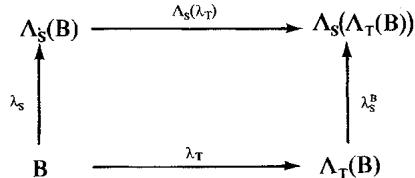
\includegraphics[keepaspectratio]{images/part001_09ec3539.jpg}}

is commutative. It suffices to check it on a generating set of the ring B.)

\begin{enumerate}
\def\labelenumi{\alph{enumi})}
\setcounter{enumi}{1}
\tightlist
\item
  Let C be a \(\lambda\)-ring, \(\rho:A \to C\) a \(\lambda\)-morphism, and \((c_i)_{i\in I}\) a family of elements of C. There exists one and only one \(\lambda\)-morphism \(\rho':B \to C\) extending \(\rho\) and such that \(\rho'(X_i) = c_i\) for all \(i\in I\).
\end{enumerate}

\begin{enumerate}
\def\labelenumi{\arabic{enumi})}
\setcounter{enumi}{51}
\tightlist
\item
  Let \((\mathbf{A}_i)_{i\in I}\) be a family of rings, \(\mathbf{A} = \prod_i\mathbf{A}_i\), and \(p_i:\mathbf{A}\to \mathbf{A}_i\) the canonical projection for every \(i\in \mathbf{I}\).\\
\end{enumerate}

\begin{enumerate}
\def\labelenumi{\alph{enumi})}
\item
  The map \(\alpha :\mathbf{A}[[T]]\to \prod_i\mathbf{A}_i[[T]]\) which maps \(\sum a_n\mathbf{T}^n\) onto \((\sum_{n}p_i(a_n)\mathbf{T}^n)_{i\in I}\) is a ring isomorphism. It defines, by restriction, a ring isomorphism \(\alpha :\Lambda (\mathbf{A})\to \prod_i\Lambda (\mathbf{A}_i)\). Moreover, we have, for all \(n\in \mathbf{J}\), \(\alpha \circ \lambda_n^{\mathbf{A}} = (\prod_i\lambda_n^{\mathbf{A}_i})\circ \alpha\) (Use the “universal polynomials” of Exerc. 46, d), p.~59.)
\item
  Suppose that, for every \(i \in I\), \(A_i\) is equipped with a structure \(\lambda_i: A_i \to \Lambda(A_i)\) of pre-\(\lambda\)-ring. By identifying \(\Lambda(A)\) with \(\prod_{i} \Lambda(A_i)\) by means of \(\alpha\), we define \(\lambda = \prod_{i} \lambda_i: A \to \Lambda(A)\). Then \((A, \lambda)\) is a pre-\(\lambda\)-ring, called the product of the family \(((A_i, \lambda_i))_{i \in I}\). For \((A, \lambda)\) to be a \(\lambda\)-ring, it is necessary and sufficient that \((A_i, \lambda_i)\) be one for all \(i \in I\).
\end{enumerate}

\begin{enumerate}
\def\labelenumi{\arabic{enumi})}
\setcounter{enumi}{52}
\tightlist
\item
  Let \(u = 1 + \mathrm{T} + \sum_{n=2}^{\infty} a_n \mathrm{T}^n\) be an element of \(\Lambda(\mathbf{Z})\). There exists one and only one group homomorphism \(\lambda^u: \mathbf{Z} \to \Lambda(\mathbf{Z})\) such that \(\lambda^u(1) = u\), and \((\mathbf{Z}, \lambda^u)\) is a pre-\(\lambda\)-ring. We have \(\lambda^u(n) = u^n\) for all \(n \in \mathbf{Z}\). For \((\mathbf{Z}, \lambda^u)\) to be a \(\lambda\)-ring, it is necessary and sufficient that \(u = 1 + \mathrm{T}\), in which case we have
\end{enumerate}

\[
\lambda_ {m} ^ {1 + \mathrm{T}} (n) = \binom {n} {m} = \frac {n (n - 1) \dots (n - m + 1)}{m !}
\]

for any \(n \in Z\) and \(m \in N\) .

\begin{enumerate}
\def\labelenumi{\arabic{enumi})}
\setcounter{enumi}{53}
\tightlist
\item
  Let C be a ring and A a C-algebra (not necessarily commutative). We denote \(\mathrm{Rep}_{\mathrm{C}}(\mathbf{A})\) the additive set of classes of A-modules that are finitely generated projective C-modules, and we denote \(\bar{\mathrm{R}}_{\mathrm{C}}(\mathring{\mathrm{A}})\) the Grothendieck group K( \(\mathrm{Rep}_{\mathrm{C}}(\mathbf{A})\) ) (cf.~A, VIII, § 10, n° 6). a) Let \(\alpha : \mathrm{A}' \to \mathrm{A}\) be a homomorphism of C-algebras. If E is an A-module of type \(\mathrm{Rep}_{\mathrm{C}}(\mathbf{A})\), then the module \(\alpha_{*}\mathrm{E}\), obtained by restriction of scalars from A to \(\mathrm{A}'\) (A, II, p.~30), is an A'-module of type \(\mathrm{Rep}_{\mathrm{C}}(\mathrm{A}')\), and {[}E{]} \(\mapsto [\alpha_{*}\mathrm{E}]\) defines a homomorphism \(\alpha_{*}: \mathrm{R}_{\mathrm{C}}(\mathrm{A}) \to \mathrm{R}_{\mathrm{C}}(\mathrm{A}')\).
\end{enumerate}

If \(\alpha_{1}:\mathbf{A}_{1}\to\mathbf{A}^{\prime}\) is a homomorphism of C-algebras, we have \((\alpha\circ\alpha_{1})_{*}=\alpha_{1*}\circ\alpha_{*}\) .

\begin{enumerate}
\def\labelenumi{\alph{enumi})}
\setcounter{enumi}{1}
\item
  One sets \(\mathbf{K}_0(\mathbf{C}) = \mathbf{R}_{\mathbf{C}}(\mathbf{C})\) . The structural homomorphism \(\varepsilon: \mathbf{C} \to \mathbf{A}\) defines a homomorphism \(\varepsilon_*: \mathbf{R}_{\mathbf{C}}(\mathbf{A}) \to \mathbf{K}_0(\mathbf{C})\) . If there exists a homomorphism \(\gamma: \mathbf{A} \to \mathbf{C}\) of C-algebras, then \(\gamma_*: \mathbf{K}_0(\mathbf{C}) \to \mathbf{R}_{\mathbf{C}}(\mathbf{A})\) is a right inverse of \(\varepsilon_*\) .
\item
  Let \(\gamma: \mathrm{C} \to \mathrm{C}'\) be a ring homomorphism. If E is an A-module of type \(\operatorname{Rep}_{\mathrm{C}}(\mathrm{A})\), then \(\gamma^{*}\mathrm{E} = \mathrm{C}' \otimes_{\mathrm{C}} \mathrm{E}\) is an \(\mathrm{A}_{\mathrm{C}'}\)-module of type \(\operatorname{Rep}_{\mathrm{C}'}(\mathrm{A}_{\mathrm{C}'})\), where \(\mathrm{A}_{\mathrm{C}'} = \mathrm{C}' \otimes_{\mathrm{C}} \mathrm{A}\), and {[}E{]} \(\mapsto [\gamma^{*}\mathrm{E}]\) defines a homomorphism \(\gamma^{*}: \mathrm{R}_{\mathrm{C}}(\mathrm{A}) \to \mathrm{R}_{\mathrm{C}'}(\mathrm{A}_{\mathrm{C}'})\). If \(\gamma_{1}': \mathrm{C}' \to \mathrm{C}_{1}\) is another ring homomorphism, we have \((\gamma_{1} \circ \gamma)^{*} = \gamma_{1}^{*} \circ \gamma^{*}\).
\item
  Let E \(\xrightarrow{f}\) F \(\xrightarrow{g}\) G be homomorphisms of A-modules, and set \(h = g \circ f\) . Construct an exact sequence of A-modules
\end{enumerate}

\[
(*) \quad 0 \rightarrow \operatorname{Ker} (f) \rightarrow \operatorname{Ker} (h) \rightarrow \operatorname{Ker} (g) \rightarrow \operatorname{Coker} (f) \rightarrow \operatorname{Coker} (h) \rightarrow \operatorname{Coker} (g) \rightarrow 0.
\]

Deduce from this that if \(f\) and \(g\) are injective, and if \(\operatorname{Coker}(f)\) and \(\operatorname{Coker}(g)\) are of type \(\operatorname{Rep}_{\mathbb{C}}(\mathbf{A})\), then \(\operatorname{Coker}(h)\) is of type \(\operatorname{Rep}_{\mathbb{C}}(\mathbf{A})\), and we have

\[
[ \operatorname{Coker} (h) ] = [ \operatorname{Coker} (f) ] + [ \operatorname{Coker} (g) ]
\]

in \(R_{C}(A)\) .

\begin{enumerate}
\def\labelenumi{\arabic{enumi})}
\setcounter{enumi}{54}
\tightlist
\item
  Let C be a ring. Let G be a monoid and let \(\mathbf{C}^{(\mathbf{G})}\) be its algebra over C. Instead of \(\mathrm{Rep}_{\mathbf{C}}(\mathbf{C}^{(\mathbf{G})})\) and \(\mathbf{R}_{\mathbf{C}}(\mathbf{C}^{(\mathbf{G})})\) , we write \(\mathrm{Rep}_{\mathbf{C}}(\mathbf{G})\) and \(\mathbf{R}_{\mathbf{C}}(\mathbf{G})\) . If \(\alpha : \mathbf{G}' \to \mathbf{G}\) is a homomorphism of monoids, we also denote by \(\alpha\) the homomorphism of C-algebras \(\mathbf{C}^{(\mathbf{G}')} \to \mathbf{C}^{(\mathbf{G})}\) that it defines, and \(\alpha_{*}: \mathbf{R}_{\mathbf{C}}(\mathbf{G}) \to \mathbf{R}_{\mathbf{C}}(\mathbf{G}')\) the corresponding homomorphism.
\end{enumerate}

By A, VIII, § 10, no. 5, there exists on R \(_{C}\) (G) a (commutative) ring structure such that

\[
[ \mathbf {E} ]. [ \mathbf {F} ] = [ \mathbf {E} \otimes_ {\mathrm{C}} \mathbf {F} ]
\]

if E and F are modules of finite type \(\mathrm{Rep}_{\mathbb{C}}(\mathbf{G})\) . The identity element for this multiplication is the class of the module \(C_1\) , equal to C with trivial action of G.

\begin{enumerate}
\def\labelenumi{\alph{enumi})}
\tightlist
\item
  The ring \(\mathbf{R}_{\mathrm{C}}(\mathbf{G})\) admits a unique structure of pre- \(\lambda\) -ring such that
\end{enumerate}

\[
\lambda [ \mathrm{E} ] = \sum_ {n \geqslant 0} \left[ \Lambda ^ {n} (\mathrm{E}) \right] \mathbf {T} ^ {n}
\]

for every module E of finite type \(\mathrm{Rep}_{\mathrm{C}}(\mathrm{G})\) . (First observe that \(\Lambda^{\mathrm{n}}(\mathrm{E})\) is again a module of finite type \(\mathrm{Rep}_{\mathrm{C}}(\mathrm{G})\) . Then, if F is a submodule such that F and E/F are of finite type \(\mathrm{Rep}_{\mathrm{C}}(\mathrm{G})\) , show that

\[
\left[ \Lambda ^ {n} (\mathrm{E}) \right] = \sum_ {p = 0} ^ {n} \left[ \Lambda ^ {p} (\mathrm{F}) \otimes_ {\mathrm{C}} \Lambda ^ {n - p} (\mathrm{E/F}) \right].
\]

in \(\mathbf{R}_{\mathbf{C}}(\mathbf{G})\).) For this, denote by \(\mathbf{L}_p\) the image of \(\Lambda^p(\mathbf{F}) \otimes_{\mathbf{C}} \Lambda^{n-p}(\mathbf{E})\), under the multiplication, in \(\Lambda^n(\mathbf{E})\). We have \(\Lambda^n(\mathbf{E}) = \mathbf{L}_0 \supset \mathbf{L}_1 \supset \ldots \supset \mathbf{L}_n = \Lambda^n(\mathbf{F}) \supset \mathbf{L}_{n+1} = 0\), and there exists a canonical isomorphism of \(\mathbf{C}^{(\mathbf{G})}\)-modules from \(\mathbf{L}_p / \mathbf{L}_{p+1}\) onto \(\Lambda^p(\mathbf{F}) \otimes \Lambda^{n-p}(\mathbf{E}/\mathbf{F})\).

\begin{enumerate}
\def\labelenumi{\alph{enumi})}
\setcounter{enumi}{1}
\item
  For every homomorphism \(\alpha: \mathbf{G}' \to \mathbf{G}\) of monoids, the map \(\alpha_*: \mathbf{R}_{\mathbf{C}}(\mathbf{G}) \to \mathbf{R}_{\mathbf{C}}(\mathbf{G}')\) is a \(\lambda\)-morphism. In particular \(\mathbf{K}_0(\mathbf{C})\) is a pre-\(\lambda\)-ring and \(\varepsilon_*: \mathbf{R}_{\mathbf{C}}(\mathbf{G}) \to \mathbf{K}_0(\mathbf{C})\) is a \(\lambda\)-morphism. The homomorphism \(\mathbf{G} \to \{1\}\) provides a right inverse for it.
\item
  Let \(\mathbf{G}\) a monoid and \(\mathbf{R}\) a set. A function \(f: \mathbf{G} \to \mathbf{R}\) will be called central if \(f(st) = f(ts)\) for any \(s, t \in \mathbf{G}\) . Let FC(G, R) denote the set of these functions. If R is a \(\lambda\) -ring, FC(G, R) is canonically endowed with a structure of \(\lambda\) -ring such that
\end{enumerate}

\[
\begin{array}{r l} (f + f ^ {\prime}) (s) & = f (s) + f ^ {\prime} (s) \\ (f \cdot f ^ {\prime}) (s) & = f (s) \cdot f ^ {\prime} (s) \\ (\lambda_ {n} f) (s) & = \lambda_ {n} (f (s)) \end{array}
\]

for any \(f, f'\) in \(\mathrm{FC}(\mathbf{G}, \mathbf{R})\) and \(s\) in \(\mathbf{G}\) . This applies in particular when \(\mathbf{R} = \Lambda(\mathbf{C})\) .

\begin{enumerate}
\def\labelenumi{\alph{enumi})}
\setcounter{enumi}{3}
\tightlist
\item
  Let E be a module of finite type \(\mathrm{Rep}_{\mathbb{C}}(\mathbf{G})\) . For every \(s \in \mathbf{G}\) , denote by \(s_{\mathbb{E}}\) the homothety of ratio \(s\) in E, and set
\end{enumerate}

\[
\overline {{{{\chi}}}} _ {\mathrm{E}} (s) = \det _ {\mathrm{E} [ \mathrm{T} ]} (1 + s _ {\mathrm{E}} \mathrm{T}) \in \Lambda (\mathrm{C})
\]

(cf. p. 62, exerc. 49). Show that

\[
\overline {{{{\chi}}}}: [ \mathrm{E} ] \mapsto \overline {{{{\chi}}}} _ {\mathrm{E}}
\]

defines a λ-morphism

\[
\overline {{{{\chi}}}}: \mathrm{R} _ {\mathrm{C}} (\mathrm{G}) \rightarrow \mathrm{FC} (\mathrm{G}, \Lambda (\mathrm{C})).
\]

\begin{enumerate}
\def\labelenumi{\alph{enumi})}
\setcounter{enumi}{4}
\tightlist
\item
  If C is a field, then \(\overline{\chi}\) is injective (A, VIII, § 10, no. 6, prop. 10). Deduce in this case that \(R_{C}(G)\) is a \(\lambda\)-ring.
\end{enumerate}

\begin{enumerate}
\def\labelenumi{\arabic{enumi})}
\setcounter{enumi}{55}
\tightlist
\item
  Let G be the free monoid generated by an element T, so that \(\mathrm{C}^{(\mathrm{G})}\) is identified with C{[}T{]}. Denote by \(C_{0}\) the module \(C{[}T{]}/T C{[}T{]}\). Then \([C_{0}]\) is an idempotent element of \(\mathrm{R}_{\mathrm{C}}(\mathrm{C}[\mathrm{T}])\). The kernel of the canonical \(\lambda\)-morphism \(\mathrm{R}_{\mathrm{C}}(\mathrm{C}[\mathrm{T}]) \rightarrow \mathrm{K}_{0}(\mathrm{C})\) is the ideal generated by \(1 - [\mathrm{C}_{0}]\). Put
\end{enumerate}

\[
\tilde {\mathrm{R}} _ {\mathrm{C}} (\mathrm{C} [ \mathrm{T} ]) = \mathrm{R} _ {\mathrm{C}} (\mathrm{C} [ \mathrm{T} ]) / [ \mathrm{C} _ {0} ]. \mathrm{R} _ {\mathrm{C}} (\mathrm{C} [ \mathrm{T} ]).
\]

\begin{enumerate}
\def\labelenumi{\alph{enumi})}
\item
  Show that \([C_{0}].R_{C}(C[T])\) is a \(\lambda\)-ideal, hence that \(\tilde{R}_{C}(C[T])\) admits a quotient pre-\(\lambda\)-ring.
\item
  For every module E of finite type \(\operatorname{Rep}_{\mathbf{C}}(\mathbf{C}[\mathbf{T}])\) , denote by \(\mathbf{T}_{\mathbf{E}}\) the homothety of ratio T in E. We have
\end{enumerate}

and

\[
\begin{array}{l} \overline {{\chi}} _ {\mathrm{E}} (\mathrm{T}) = \det _ {\mathrm{E} [ \mathrm{T} ]} (1 + \mathrm{T} _ {\mathrm{E}} \mathrm{T}) \in \Lambda (\mathrm{C}) \\ \chi_ {\mathrm{E}} (\mathrm{T}) = \det _ {\mathrm{E} [ \mathrm{T} ]} (\mathrm{T} - \mathrm{T} _ {\mathrm{E}}) \end{array}
\]

is the characteristic polynomial of \(T_{E}\) (cf.~exerc. 49, p.~62). Show that \([E] \mapsto \overline{\chi}_{E}(T)\) defines a \(\lambda\) -morphism \(R_{C}(C[T]) \to \Lambda(C)\) whose kernel contains \([C_{0}]\) . By passing to the quotient, we obtain a \(\lambda\) -morphism

\[
\overline {{\chi}}: \tilde {\mathrm{R}} _ {\mathrm{C}} (\mathrm{C} [ \mathrm{T} ]) \to \Lambda (\mathrm{C}).
\]

\begin{enumerate}
\def\labelenumi{\alph{enumi})}
\setcounter{enumi}{2}
\item
  Denote by \(\Lambda_{\mathrm{rat}}(\mathbf{C})\) the subgroup of \(\Lambda(\mathbf{C})\) generated by the elements of \(\Lambda(\mathbf{C})\) which are polynomials in T. Show that the image of \(\overline{\chi}\) is \(\Lambda_{\mathrm{rat}}(\mathbf{C})\). Conclude from this that \(\Lambda_{\mathrm{rat}}(\mathbf{C})\) is a sub-\(\lambda\)-ring of \(\Lambda(\mathbf{C})\).
\item
  For every \(r \in \mathbf{Z}\), define \(\sigma_r: \mathrm{C}[\mathrm{T}, \mathrm{T}^{-1}] \to \mathrm{C}[\mathrm{T}, \mathrm{T}^{-1}]\) by \((\sigma_r f)(\mathrm{T}) = \mathrm{T}^{r} f((-\mathrm{T})^{-1})\). We have \((\sigma_r(\sigma_s f))(\mathrm{T}) = (-1)^s \mathrm{T}^{r-s} f(\mathrm{T})\), in particular \(\sigma_r(\sigma_r f) = (-1)^r f\), and \((\sigma_r f).(\sigma_s g) = \sigma_{r+s}(f.g)\), for all \(r, s\) in \(\mathbf{Z}\) and \(f, g\) in \(\mathrm{C}[\mathrm{T}, \mathrm{T}^{-1}]\). If \(f\) is a polynomial in \(T\) of degree \(\leqslant r\) (\(r \geqslant 0\)), then \(\sigma_r f\) is one as well. If moreover \(f \in \Lambda(\mathrm{C})\) (i.e. \(f(0) = 1\)), then \(\sigma_r f\) is monic of degree \(r\). If E is a C{[}T{]}-module which is a free C-module of rank \(r\), one has \(\sigma_r(\overline{\chi}_{\mathrm{E}}(\mathrm{T})) = \chi_{\mathrm{E}}(\mathrm{T})\). e) If \(f \in \Lambda(\mathrm{C})\) is a polynomial in \(T\) of degree \(\leqslant r\), set \(E_{r,f} = C[T]/\sigma_r f.C[T]\); it is a free C-module of rank \(r\). If \(f = 1\) we have \(E_{r,1} = C[T]/T^{r}C[T]\). If \(g \in \Lambda(\mathrm{C})\) is a polynomial in \(T\) of degree \(\leqslant s\), we have an exact sequence of C{[}T{]}-modules
\end{enumerate}

\[
(*) \quad 0 \rightarrow \mathrm{E} _ {s, g} \rightarrow \mathrm{E} _ {r + s, f g} \rightarrow \mathrm{E} _ {r, f} \rightarrow 0
\]

(using \(d\) ). Show that the class \(\tau(f)\) of \(\mathrm{E}_{r,f}\) in \(\tilde{\mathrm{R}}_{\mathrm{C}}(\mathrm{C}[\mathrm{T}])\) is independent of \(r\) ( \(\geqslant \deg(f)\) ). (Indeed \(\sigma_{r+s}f = (\sigma_s1).(\sigma_rf) = \mathrm{T}^s.(\sigma_rf)\) and the class of the module \(\mathrm{C}[\mathrm{T}] / \mathrm{T}^s\mathrm{C}[\mathrm{T}]\) in \(\tilde{\mathrm{R}}_{\mathrm{C}}(\mathrm{C}[\mathrm{T}])\) is zero.) Show that if \(g\) is a polynomial in \(\Lambda(\mathrm{C})\) , one has \(\tau(fg) = \tau(f) + \tau(g)\) . (Use again the exact sequence (*).) Deduce from this that \(\tau\) extends to a group homomorphism

\[
\tau : \Lambda_ {\mathrm{rat}} (\mathrm{C}) \rightarrow \tilde {\mathrm{R}} _ {\mathrm{C}} (\mathrm{C} [ \mathrm{T} ]).
\]

\begin{enumerate}
\def\labelenumi{\alph{enumi})}
\setcounter{enumi}{5}
\tightlist
\item
  Show that \(\overline{\chi} \circ \tau\) is the identity map of \(\Lambda_{\mathrm{rat}}(\mathbf{C})\) (Using the fact that if \(f \in \Lambda(\mathbf{C})\) is a polynomial of degree \(\leqslant r\), then the characteristic polynomial of \(\mathrm{T}_{\mathrm{E}_r,f}\) is \(\sigma_r f\).)
\item
  Show that every element of \(\tilde{\mathrm{R}}_{\mathrm{C}}(\mathrm{C}[\mathrm{T}])\) is the class of a C{[}T{]}-module E which is a free C-module.
\end{enumerate}

\(h\) ) Let E be a C{[}T{]}-module, and denote by \(u\in \mathrm{End}_{\mathrm{C}}(\mathrm{E})\) the homothety of ratio T in E; let \(\overline{u} = \mathrm{Id}_{\mathrm{C[T]}}\otimes_{\mathrm{C}}u\in \mathrm{End}_{\mathrm{C[T]}}(\mathrm{E}[\mathrm{T}])\). We have an exact sequence of C{[}T{]}-modules

\[
0 \longrightarrow \mathrm{E} [ \mathrm{T} ] \xrightarrow {\mathrm{T} - \bar {u}} \mathrm{E} [ \mathrm{T} ] \longrightarrow \mathrm{E} \longrightarrow 0
\]

(A, III, p.~106). Suppose that E is a free C-module with basis \((e_1, \ldots, e_r)\). Then E{[}T{]} is a free C{[}T{]}-module with basis \((1 \otimes e_i)\). If the matrix of \(u\) for the basis \((e_i)\) is \((a_{ij})\), the matrix of T - \(\overline{u}\) for the basis \((1 \otimes e_i)\) is \((\mathrm{T}\delta_{ij} - a_{ij})\).

\begin{enumerate}
\def\labelenumi{\roman{enumi})}
\tightlist
\item
  Let \(f = (f_{ij})_{1 \leqslant i,j \leqslant r}\) be a matrix with coefficients in C{[}T{]}. We say that \(f\) is special if, for all \(i, j\) in \(\{1, \dots, r\}\), \(i \neq j\), \(f_{ii}\) is a monic polynomial and \(\deg(f_{ii}) > \deg(f_{ij})\). Then show that \(\det(f)\) is a monic polynomial (of degree \(\deg(f_{11}) + \cdots + \deg(f_{rr})\)) and that \(f\) defines an injective endomorphism of C{[}T{]} \(^r\). Deduce from h) that every C{[}T{]}-module which is a free C-module of rank \(r\) is isomorphic to the cokernel of such an endomorphism of C{[}T{]} \(^r\).
\end{enumerate}

\begin{enumerate}
\def\labelenumi{\alph{enumi})}
\setcounter{enumi}{9}
\tightlist
\item
  Let f be a special matrix as in i). Set \(f = \begin{pmatrix} f_{11} & f_{+} \\ f_{-} & f' \end{pmatrix}\) where \(f_{+}\) , \(f_{-}\) , \(f'\) are matrices of types \((1, r - 1)\) , \((r - 1, 1)\) and \((r - 1, r - 1)\) respectively. Set
\end{enumerate}

\[
g = \left( \begin{array}{c c} 1 & 0 \\ - f _ {-} & f _ {1 1} \mathrm{I} \end{array} \right) \quad \text {and} \quad h = g f = \left( \begin{array}{c c} f _ {1 1} & f _ {+} \\ 0 & \overline {{f}} \end{array} \right) \quad \text {where} \quad \overline {{f}} = f _ {1 1} f ^ {\prime} - f _ {-} f _ {+}.
\]

Show that h is a special matrix. Moreover, by identifying square matrices with the corresponding endomorphisms, one obtains exact sequences of C{[}T{]}-modules

\[
0 \rightarrow \operatorname{Coker} (f) \rightarrow \operatorname{Coker} (h) \rightarrow \operatorname{Coker} (g) \rightarrow 0,
\]

(where Coker(g) is isomorphic to \(\mathbf{C}[\mathbf{T}]^{r - 1} / f_{11}\mathbf{C}[\mathbf{T}]^{r - 1}\) ) and

\[
0 \rightarrow \mathrm{C} [ \mathrm{T} ] / f _ {1 1} \mathrm{C} [ \mathrm{T} ] \rightarrow \operatorname{Coker} (h) \rightarrow \operatorname{Coker} (\bar {f}) \rightarrow 0.
\]

From this, deduce by induction on \(r\) that \(\operatorname{Coker}(f)\) is a projective C-module whose class in \(\mathbf{R}_{\mathrm{C}}(\mathbf{C}[\mathrm{T}])\) is a \(\mathbf{Z}\)-linear combination of elements of the form \([\mathbf{C}[\mathrm{T}] / p\mathbf{C}[\mathrm{T}]]\), where \(p\) is a monic polynomial.

  \(k\) ) Use parts \(f\), \(g\), \(i)\), and \(j)\) above to show that \(\tau : \Lambda_{\mathrm{rat}}(\mathbf{C}) \to \tilde{\mathbf{R}}_{\mathrm{C}}(\mathbf{C}[\mathrm{T}])\) is surjective, hence that \(\overline{\chi} : \tilde{\mathbf{R}}_{\mathrm{C}}(\mathbf{C}[\mathrm{T}]) \to \Lambda_{\mathrm{rat}}(\mathbf{C})\) is an isomorphism.

\begin{enumerate}
\def\labelenumi{\alph{enumi})}
\setcounter{enumi}{11}
\tightlist
\item
  Show that \(\Lambda_{\mathrm{rat}}(\mathbf{C})\) is stable under \(\mathbf{V}_n\) and \(\mathbf{F}_n\) for each \(n \in \mathbf{J}\). There therefore correspond to them endomorphisms \(\mathbf{V}_n\) and \(\mathbf{F}_n\) of \(\tilde{\mathbf{R}}_{\mathbf{C}}(\mathbf{C}[\mathbf{T}])\), by the preceding isomorphism. Let \(\varphi_n\) be the homomorphism of C-algebras from C{[}T{]} to itself which maps T to \(\mathbf{T}^n\). Show that \(\mathbf{V}_n\) (resp. \(\mathbf{F}_n\)) is deduced from the endomorphism \(\varphi_n^*\) (resp. \((\varphi_n)_*\)) of \(\mathbf{R}_{\mathbf{C}}(\mathbf{C}[\mathbf{T}])\) by passing to quotients.
\end{enumerate}

In the following exercises, p is a fixed prime number, and the rings of Witt vectors are relative to this prime number.

\begin{enumerate}
\def\labelenumi{\arabic{enumi})}
\setcounter{enumi}{56}
\tightlist
\item
  Let \(m\), \(n\) be two integers \(\geqslant 1\). For every ring A of characteristic \(p\), denote by \(_{m}\mathrm{W}_{n}(\mathrm{A})\) the kernel of the endomorphism \(\mathrm{F}^{m}\) of \(\mathrm{W}_{n}(\mathrm{A})\).
\end{enumerate}

\begin{enumerate}
\def\labelenumi{\alph{enumi})}
\tightlist
\item
  For \(m \geqslant 2\) and \(n \geqslant 1\) the following diagram is commutative
\end{enumerate}

\pandocbounded{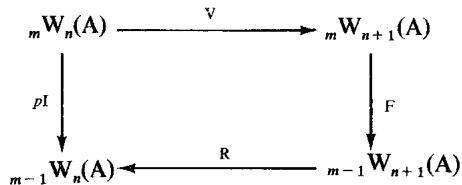
\includegraphics[keepaspectratio]{images/part001_6a9997c3.jpg}}

where the maps V, F are induced by the shift and Frobenius homomorphisms, respectively, I is the natural injection, and R is the natural projection.

\begin{enumerate}
\def\labelenumi{\alph{enumi})}
\setcounter{enumi}{1}
\tightlist
\item
  For \(n \geqslant 1\) and \(a = [a_0, \ldots, a_{n-1}]\) in \(W_n(A)\) , denote by \(\tilde{a}\) the element \((a_0, \ldots, a_{n-1}, 0, \ldots)\) of \(W(A)\) .
\end{enumerate}

Let \(a \in_{m} W_{n}(A)\) , \(b \in_{n} W_{m}(A)\) We then set

\[
\langle \boldsymbol {a}, \boldsymbol {b} \rangle = \mathrm{E} (\omega_ {\mathrm{A}} (\tilde {\boldsymbol {a}}) \omega_ {\mathrm{A}} (\tilde {\boldsymbol {b}}), 1)
\]

(cf. p. 57, exerc. 43 for the notation E, and p. 54, exerc. 40 for the notation \(\omega_{\mathbf{A}}\) ). Prove that the map \((\boldsymbol{a}, \boldsymbol{b}) \mapsto \langle \boldsymbol{a}, \boldsymbol{b} \rangle\) from \({}_{m}W_n(A) \times {}_{n}W_m(A)\) into \(A^*\) is \(\mathbf{Z}\)-bilinear. c) With the notation of a), we have

\[
\langle \boldsymbol {a}, \mathrm{V} \boldsymbol {b} \rangle = \langle \mathrm{F} \boldsymbol {a}, \boldsymbol {b} \rangle . \text { for } \quad \boldsymbol {a} \in_ {m} \mathrm{W} _ {n} (\mathrm{A}) \quad \text { and } \quad \boldsymbol {b} \in_ {n} \mathrm{W} _ {m - 1} (\mathrm{A})
\]

and

\[
\langle \mathbf {R} \boldsymbol {a}, \boldsymbol {b} \rangle = \langle \boldsymbol {a}, \mathbf {I} \boldsymbol {b} \rangle \quad \text { for } \quad \boldsymbol {a} \in_ {m} \mathrm{W} _ {n} (\mathrm{A}) \quad \text { and } \quad \boldsymbol {b} \in_ {n - 1} \mathrm{W} _ {m} (\mathrm{A}).
\]

\begin{enumerate}
\def\labelenumi{\arabic{enumi})}
\setcounter{enumi}{57}
\tightlist
\item
  \begin{enumerate}
  \def\labelenumii{\alph{enumii})}
  \tightlist
  \item
    Let \(\delta(T)\) be the formal series \(\exp\left(-\sum_{n=0}^{\infty}\mathrm{T}^{p^n}/p^n\right)\) of \(\mathbf{Q}[[T]]\). We have
  \end{enumerate}
\end{enumerate}

\[
\mathfrak{E}(\mathrm{T}) = \prod_{\substack{(n,p) = 1\\ n\text{ an integer}\geqslant 1}}(1 - \mathrm{T}^{n})^{\mu (n) / n}
\]

where μ is the Möbius function. The coefficients of δ(T) belong to \(\mathbf{Z}_{(p)}\). b) Let \(\mathbf{X} = (\mathbf{X}_{n})_{n \in \mathbb{N}}\) be a family of indeterminates. In the algebra \(\mathbf{Q}[(\mathbf{X}_{n})_{n \in \mathbb{N}}]\), we have the equality

\[
\prod_ {n = 0} ^ {\infty} \mathcal {E} (\mathrm{X} _ {n} \mathrm{T} ^ {p ^ {n}}) = \exp \left(- \sum_ {n = 0} ^ {\infty} \Phi_ {n} (\mathrm{X}) \mathrm{T} ^ {p ^ {n}} / p ^ {n}\right).
\]

\begin{enumerate}
\def\labelenumi{\alph{enumi})}
\setcounter{enumi}{2}
\item
  Let A be a \(\mathbf{Z}_{(p)}\) -algebra. It is assumed that multiplication by \(p, 1_{\mathbf{A}}\) is injective in A. Let \(\boldsymbol{a} = (a_n)_{n \in \mathbb{N}} \in \mathbb{A}^{\mathbf{N}}\) . For the series \(\exp\left(\sum_{n=0}^{\infty} a_n \mathbf{T}^{p^n} / p^n\right)\) of \(\mathrm{A}\left[\frac{1}{p}\right]\) {[}{[}T{]}{]} to have its coefficients in A, it is necessary and sufficient that \(\boldsymbol{a}\) belongs to \(\Phi_{\Lambda}(\mathbf{W}(\mathbf{A}))\) .
\item
  Let A be a \(\mathbf{Z}_{(p)}\)-algebra. The map \(\mathbf{E} \circ \omega_{\Lambda}\) from W(A) to \(\Lambda(\mathbf{A})\) (cf.~p.~54, exerc. 40 and p.~57, exerc. 43) associates to \(\boldsymbol{a} = (a_n)_{n \in \mathbb{N}}\) the element \(\prod_{n=0}^{\infty} \delta(a_n(-\mathbf{T})^{p^n})\) of \(\Lambda(\mathbf{A})\).
\item
  Let A be a \(\mathbf{Z}_{(p)}\)-algebra. Suppose that multiplication by \(p,1_{A}\) is injective in A. Let \(\sigma\) be an endomorphism of A satisfying \(\sigma a \equiv a^{p} \mod pA\). Let \(s_{\sigma}:A \to W(A)\) be the homomorphism associated with \(\sigma\) (p.~44, exerc. 14). Then, for every \(a \in A\), the formal series
\end{enumerate}

\[
\mathrm{E} _ {\sigma} (a, \mathrm{T}) = \exp (\sum_ {i = 0} ^ {\infty} \sigma^ {i} (a) \mathrm{T} ^ {p ^ {i}} / p ^ {i})
\]

has its coefficients in A, and we have

\[
\mathrm{E} \circ \omega_ {\mathrm{A}} \circ s _ {\sigma} (a ^ {- 1}) = \exp \left(\sum_ {i = 0} ^ {\infty} \sigma^ {i} (a) (- \mathrm{T}) ^ {p ^ {i}} / p ^ {i}\right) = \mathrm{E} _ {\sigma} (a, - \mathrm{T}).
\]

\begin{enumerate}
\def\labelenumi{\alph{enumi})}
\setcounter{enumi}{5}
\tightlist
\item
  Let \(\mathcal{A}\) the ring \(\mathbf{Z}_{(p)}[(\mathbf{X}_n)_{n\in\mathbb{N}}]\) and let \(\mathbf{X} = (\mathbf{X}_n)_{n\in\mathbb{N}} \in \mathrm{W}(\mathcal{A})\) . The series \(\mathrm{E}_{\mathrm{F},\mathcal{A}}(\mathbf{X},\mathrm{T})\) has its coefficients in \(\mathrm{W}(\mathcal{A})\) . For every \(\mathbf{Z}_{(p)}\) -algebra A and every element \(a = (a_n)_{n\in\mathbb{N}}\) of \(\mathrm{W}(\mathrm{A})\) , we shall write \(\mathrm{E}_{\mathrm{F}}(a,\mathrm{T})\) the series obtained by applying \(\mathrm{W}(\varphi)\) to the coefficients of \(\mathrm{E}_{\mathrm{F},\mathcal{A}}(\mathbf{X},\mathrm{T})\) where \(\varphi: \mathcal{A} \to \mathrm{A}\) is the map which to \(\mathrm{X}_n\) to \(a_n\) . Then \(\mathrm{E}_{\mathrm{F}}(a,\mathrm{T})\) has its coefficients in \(\mathrm{W}(\mathrm{A})\) and if \(s_{\mathrm{A}}\) denotes the homomorphism \(\mathrm{W}(\mathrm{A}) \to \mathrm{W}(\mathrm{W}(\mathrm{A}))\) defined in Exerc. 15, p.~44, we have
\end{enumerate}

\[
\mathrm{E} \circ \omega_ {\mathrm{W(A)}} \circ s _ {\mathrm{A}} (\boldsymbol {a} ^ {- 1}) = \mathrm{E} _ {\mathrm{F}} (\boldsymbol {a}, - \mathrm{T}) \quad \text { for all } \quad \boldsymbol {a} \in \mathrm{W(A)}.
\]

\exercisesection{COHEN RINGS}

In the exercises of § 2, \(p\) is a fixed prime number. If \(a\) is an ideal of a ring A, we denote by \(a^p\) the ideal generated by the elements \(a^p\) , where \(a\) ranges over \(a\) .

\begin{enumerate}
\def\labelenumi{\arabic{enumi})}
\item
  Let \((\mathbf{C}_{n}, \pi_{n,m})\) be a projective system of rings relative to the index set N. We assume that \(C_{n}\) is Artinian for every \(n \in N\) and that the homomorphisms \(\pi_{n,m}\) are surjective. Let \(\pi_{n}\) be the canonical homomorphism from \(C = \varprojlim C_{n}\) into \(C_{n}\). Show that for all \(x \in C\), one has \(xC = \varprojlim \pi_{n}(x) C_{n}\). (Proceed as in the proof of Prop. 3 of § 2, no. 1.)
\item
  Let A be a ring and \((\mathbf{J}_{n})_{n\in\mathbb{N}}\) a decreasing sequence of ideals of A, such that \(pJ_{n} + J_{n}^{p} \subset J_{n+1}\) for every \(n \in N\).
\end{enumerate}

\begin{enumerate}
\def\labelenumi{\alph{enumi})}
\item
  Prove that the assertions of Lemma 1 and Prop. 1 of § 1, no. 1 are still true under this hypothesis.
\item
  Let \(i\) and \(n\) be two positive integers. When \(i \leqslant n\), the map \(x \mapsto p^i x^{p^n - i}\) from A to A defines, by passing to quotients, a map
\end{enumerate}

\[
\rho_ {n, i} ^ {\mathbf {A}}: \mathrm{A} / \mathrm{J} _ {0} \rightarrow \mathrm{A} / \mathrm{J} _ {n}.
\]

For \(i > n\) , we set \(\rho_{n,i}^{\mathbf{A}} = 0\) . For \(x \in \mathrm{A} / \mathrm{J}_n\) and \(a \in \mathrm{A} / \mathrm{J}_0\) , one has \(x^{p^{n - i}} \rho_{n,i}^{\mathbf{A}}(a) = \rho_{n,i}^{\mathbf{A}}(\overline{x} a)\) , where \(\overline{x}\) is the image of \(x\) in \(\mathrm{A} / \mathrm{J}_0\) . If \(j\) is a positive integer and that \(a, b\) are two elements of \(\mathrm{A} / \mathrm{J}_n\) , one has

\[
\rho_ {n, i} ^ {\mathbf {A}} (a) \rho_ {n, j} ^ {\mathbf {A}} (b) = \rho_ {n, i + j} ^ {\mathbf {A}} \left(a ^ {p ^ {j}} b ^ {p ^ {i}}\right).
\]

\begin{enumerate}
\def\labelenumi{\alph{enumi})}
\setcounter{enumi}{2}
\tightlist
\item
  Let \((\mathbf{R}_{n})_{n\in\mathbf{N}}\) be the sequence of polynomials constructed in exerc. 3, p.~42. Let n and i be two positive integers, and let a and b be two elements of \(A/J_{0}\). We then have, in \(A/J_{n}\), the equality
\end{enumerate}

\[
\rho_ {n, i} ^ {\mathrm{A}} (a) + \rho_ {n, i} ^ {\mathrm{A}} (b) = \sum_ {m = 0} ^ {n - i} \rho_ {n, i + m} ^ {\mathrm{A}} (\mathrm{R} _ {m} (a, b)).
\]

\begin{enumerate}
\def\labelenumi{\arabic{enumi})}
\setcounter{enumi}{2}
\tightlist
\item
  Let \(n\) be a positive integer. Let C be a \(p\)-Cohen ring, with residue field \(k\), and of length \(n+1\). Let \((x_{\lambda})_{\lambda\in\Lambda}\) be a family of elements of C lifting a \(p\)-basis \((\xi_{\lambda})_{\lambda\in\Lambda}\) of \(k\). We denote by \(\rho_{i}:k\to C\), for every \(i\in\mathbf{N}\), the map \(\rho_{n,i}^{\mathrm{C}}\) defined in Exerc. 2, where one takes for \(\mathbf{J}_{m}\) the ideal \(p^{m+1}\mathbf{C}\).
\end{enumerate}

\begin{enumerate}
\def\labelenumi{\alph{enumi})}
\tightlist
\item
  For \(r \in \mathbf{N}\), let \(\mathbf{M}_r\) be the set of multi-indices \(m \in \mathbf{N}^{(\Lambda)}\) such that, for every \(\lambda \in \Lambda\), one has \(0 \leqslant m_{\lambda} < p^{r}\). Then, for every element \(\alpha\) of C, there exists a unique finitely supported family \((a_{i,m})\) (\(0 \leqslant i \leqslant n\), \(m \in \mathbf{M}_{n-i}\)) of elements of \(k\), such that
\end{enumerate}

\[
\alpha = \sum_ {i = 0} ^ {n} \sum_ {m \in \mathbf {M} _ {n - i}} \rho_ {i} (a _ {i, m}) x ^ {m},
\]

where the notation \(x^{m}\) denotes the product \(\prod x_{\lambda}^{m_{\lambda}}\) .

\begin{enumerate}
\def\labelenumi{\alph{enumi})}
\setcounter{enumi}{1}
\tightlist
\item
  Consider the ring U generated by the generators \([x_{\lambda}]\), with \(\lambda\) ranging over \(\Lambda\), and \([\rho_{i}(a)]\), with i ranging over N and a ranging over k, and subject only to the following relations (where the polynomials \(R_{i}\) are those introduced in Exerc. 3, p.~42).
\end{enumerate}

\begin{enumerate}
\def\labelenumi{(\roman{enumi})}
\item
  \([\rho_i(a)] = 0\) for \(a \in k, i > n\) ,
\item
  \(\left[\rho_0(1)\right] = 1\) and \(\left[\rho_0(0)\right] = 0,\)
\item
  \([\rho_i(a)][\rho_j(b)] = [\rho_{i + j}(a^{p^j}b^{p^i})]\) for \(i,j\) in \(\mathbf{N}\) and \(a,b\) in \(k\) ,
\item
  \([\rho_i(a)] + [\rho_i(b)] = \sum [\rho_{i+m}(\mathbf{R}_m(a,b))]\) for \(i\in \mathbf{N}\) and \(a,b\) in \(k,\)
\item
  \([x_{\lambda}]^{p^{n - i}}[\rho_i(a)] = [\rho_i(\xi_{\lambda}a)]\) for \(0 \leqslant i \leqslant n, \lambda \in \Lambda, a \in k\) .
\end{enumerate}

Prove that we have \([\rho_i(0)] = 0\) for every \(i \in \mathbf{N}\) .

Prove, using exercise 3, b), p.~42, that if \(p\) is odd, we have \([\rho_0(-1)] = -1\) ; if \(p\) is even, we have \(\sum_{i=0}^{n} [\rho_i(1)] = -1\) .

\begin{enumerate}
\def\labelenumi{\alph{enumi})}
\setcounter{enumi}{2}
\tightlist
\item
  There exists a unique map from U to C which, for every finitely supported family \((a_{i,m})_{0\leqslant i\leqslant n,m\in M_{n - i}}\) of elements of \(k\) associated with the element
\end{enumerate}

\[
\left\langle \left(a _ {i, m}\right) \right\rangle = \sum_ {i = 0} ^ {n} \sum_ {m \in \mathbf {M} _ {n - i}} \left[ \rho_ {i} (a _ {i, m}) \right] \prod_ {\lambda \in \Lambda} [ x _ {\lambda} ] ^ {m _ {\lambda}}
\]

of U the element \(\sum_{i=0}^{n}\sum_{m\in M_{n-i}}\rho_i(a_{i,m})x^m\) of C; it is a ring isomorphism.

\begin{enumerate}
\def\labelenumi{\alph{enumi})}
\setcounter{enumi}{3}
\tightlist
\item
  Deduce from the foregoing another proof of the results of § 2, no. 3.
\end{enumerate}

\begin{enumerate}
\def\labelenumi{\arabic{enumi})}
\setcounter{enumi}{3}
\tightlist
\item
  Let C be a \(p\)-Cohen ring of infinite length, and \(k\) its residue field. Let A be a ring, and \((\mathbf{J}_n)_{n \in \mathbb{N}}\) a decreasing sequence of ideals of A satisfying \(p\mathbf{J}_n + \mathbf{J}_n^p \subset \mathbf{J}_{n+1}\) for every \(n \in \mathbb{N}\). Finally, let \(\overline{\varphi}: k \to \mathrm{A} / \mathrm{J}_0\) be a ring homomorphism, \((\xi_\lambda)_{\lambda \in \Lambda}\) a \(p\)-basis of \(k\), \((x_\lambda)_{\lambda \in \Lambda}\) a family of elements of C lifting this \(p\)-basis, and \((a_\lambda)_{\lambda \in \Lambda}\) a family of elements of A, such that the image of \(a_\lambda\) in \(\mathrm{A} / \mathrm{J}_0\) is \(\overline{\varphi}(\xi_\lambda)\).
\end{enumerate}

\begin{enumerate}
\def\labelenumi{\alph{enumi})}
\item
  For every \(n\in\mathbf{N}\), there exists a unique homomorphism \(\varphi_{n}\) from \(\mathrm{C}/p^{n+1}\mathrm{C}\) into \(\mathrm{A}/\mathrm{J}_{n}\) such that \(\varphi_{n}\circ\rho_{n,i}^{\mathrm{C}}=\rho_{n,i}^{\mathrm{A}}\circ\overline{\varphi}\) and such that the image under \(\varphi_{n}\) of the class of \(x_{\lambda}\) is the class of \(a_{\lambda}\) (Use Exercises 2 and 3.)
\item
  Suppose that A is separated and complete for the topology defined by the filtration \((\mathrm{J}_{n})_{n\in\mathbb{N}}\). Then there exists a unique ring homomorphism \(\varphi\) from C to A, such that \(\varphi(x_{\lambda}) = a_{\lambda}\) for \(\lambda \in \Lambda\), and that \(\varphi\) induces \(\overline{\varphi}\) by passing to quotients. This homomorphism is continuous.
\item
  Suppose that the ring A is local, separated, and complete, that one has \(J_{n} = m_{A}^{n+1}\) for every \(n \in N\), that one has \(A/J_{0} = k\), and that \(\overline{\varphi}\) is the identity map. Prove that the image under \(\varphi\) of C in A is the unique Cohen subring of \(A'\) containing each of the elements \(a_{\lambda}\), and thus give another proof of part a) of th. 1 of § 2, no. 2; if k is perfect and C is the ring W(k), one obtains another proof of th. 2 of § 2, no. 4.
\end{enumerate}

\begin{enumerate}
\def\labelenumi{\arabic{enumi})}
\setcounter{enumi}{4}
\tightlist
\item
  Let A be a ring and \((\mathrm{J}_n)_{n\in \mathbb{N}}\) a decreasing sequence of ideals of A, satisfying \(p\mathbf{J}_n + \mathbf{J}_n^p\subset \mathbf{J}_{n + 1}\) for every integer \(n\geqslant 0\). Let R be a ring of characteristic \(p\) and \(\overline{\varphi}\) a ring homomorphism from R to \(\mathrm{A} / \mathrm{J}_0\). One calls a lifting of \(\overline{\varphi}\) into \(\mathrm{A} / \mathrm{J}_n\) a map \(\varphi_n:\mathbb{R}\to \mathbb{A} / \mathbb{J}_n\) such that \(\varphi_n(x^p) = \varphi_n(x)^p\) for \(x\in \mathbb{R}\), and which gives back \(\overline{\varphi}\) by passing to the quotient. a) Let \(\varphi_n\) and \(\widetilde{\varphi}_n\) be two lifts of \(\overline{\varphi}\) into \(\mathrm{A} / \mathrm{J}_n\). Then \(\varphi_n\) and \(\widetilde{\varphi}_n\) coincide on \(\mathbb{R}^{p^n}\). b) If R is perfect, there exists a unique lift \(\varphi_n\) of \(\overline{\varphi}\) into \(\mathrm{A} / \mathrm{J}_n\). We have \(\varphi_n(1) = 1\) and \(\varphi_n(xy) = \varphi_n(x)\varphi_n(y)\), for \(x,y\in \mathbb{R}\).
\end{enumerate}

\begin{enumerate}
\def\labelenumi{\arabic{enumi})}
\setcounter{enumi}{5}
\tightlist
\item
  Let A be a ring and \((\mathbf{J}_{n})_{n\in\mathbb{N}}\) a decreasing sequence of ideals of A. We assume that A is separated and complete for the topology defined by the filtration \((\mathbf{J}_{n})_{n\in\mathbb{N}}\) and that one has \(pJ_{n} + J_{n}^{p} \subset J_{n+1}\) for every integer \(n \geqslant 0\). We denote \(\pi_{n}\) the canonical map from A onto \(A/J_{n}\). Let R be a perfect ring of characteristic p and \(\overline{\varphi}\) a ring homomorphism from R to \(A/J_{0}\).
\end{enumerate}

\begin{enumerate}
\def\labelenumi{\alph{enumi})}
\item
  There exists a unique map \(\varphi\) from R into A such that one has \(\overline{\varphi} = \pi_0 \circ \varphi\) and \(\varphi(x^p) = \varphi(x)^p\) for every \(x \in \mathbb{R}\). Moreover, we have \(\varphi(1) = 1\) and \(\varphi(xy) = \varphi(x)\varphi(y)\) for \(x\) and \(y\) in R. When A is a ring of characteristic \(p\), \(\varphi\) is a ring homomorphism. (One may use the preceding exercise.)
\item
  For every \(n\in\mathbf{N}\) there exists a unique ring homomorphism \(v_{n}:W_{n+1}(A/J_{0})\to A/J_{n}\) thereby making the diagram commutative
\end{enumerate}

\pandocbounded{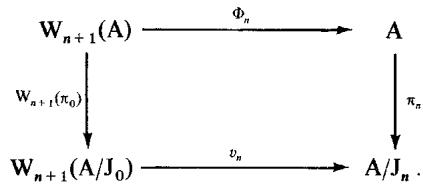
\includegraphics[keepaspectratio]{images/part002_309b7be5.jpg}}

\begin{enumerate}
\def\labelenumi{\alph{enumi})}
\setcounter{enumi}{2}
\tightlist
\item
  Set \(u_n = v_n \circ \mathbf{W}_{n+1}(\overline{\varphi}) \circ \mathbf{F}^{-n}\) Then, for every \(n \in \mathbf{N}\) , the following diagram, where the vertical arrows denote the canonical projections, is commutative
\end{enumerate}

\pandocbounded{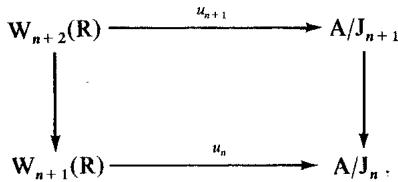
\includegraphics[keepaspectratio]{images/part002_feb0ecf4.jpg}}

\begin{enumerate}
\def\labelenumi{\alph{enumi})}
\setcounter{enumi}{3}
\tightlist
\item
  There exists a unique ring homomorphism u making the following diagram commutative.
\end{enumerate}

\pandocbounded{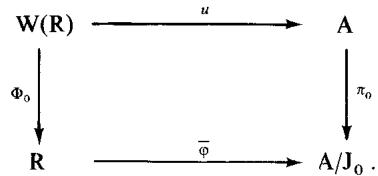
\includegraphics[keepaspectratio]{images/part002_890d1cac.jpg}}

  The homomorphism \(u\) is continuous when \(\mathbf{W}(\mathbf{R})\) is equipped with the \(p\)-adic topology, and for every \(\boldsymbol{a} = (a_n)_{n \in \mathbb{N}} \in \mathbf{W}(\mathbf{R})\), one has \(u(\boldsymbol{a}) = \sum_{n=0}^{\infty} p^n \varphi(a_n^{p^{-n}})\).

(The existence of \(u\) follows from what precedes. To prove the uniqueness of \(u\), its continuity, and its explicit expression, use the equality \(\varphi = u \circ \tau\), where \(\varphi\) is the map from R into A constructed in a), and \(\tau: \mathrm{R} \to \mathrm{W(R)}\) is the map defined in § 1, no. 5.)

\begin{enumerate}
\def\labelenumi{\alph{enumi})}
\setcounter{enumi}{4}
\tightlist
\item
  Give another proof of th. 2 of § 2, no. 4, different from the one in the text and from that of exerc. 4, c).
\end{enumerate}

\begin{enumerate}
\def\labelenumi{\arabic{enumi})}
\setcounter{enumi}{6}
\tightlist
\item
  \begin{enumerate}
  \def\labelenumii{\alph{enumii})}
  \tightlist
  \item
    Let R be a perfect ring of characteristic p, and let R' be a ring of characteristic p. Let f be a homomorphism from R into R'. Then the homomorphism W(f): W(R) → W(R') is the unique homomorphism making the following diagram commutative.
  \end{enumerate}
\end{enumerate}

\pandocbounded{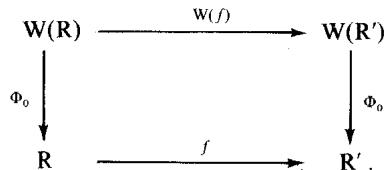
\includegraphics[keepaspectratio]{images/part002_f36acea2.jpg}}

(Use the previous exercise.)

In particular, taking \(f\) to be the p-th power map on R, prove that \(\mathrm{F}_{\mathrm{R}}\) is the unique endomorphism of \(\mathbf{W}(\mathbf{R})\) such that \(\Phi_{0} \circ \mathrm{F}_{\mathrm{R}} = f \circ \Phi_{0}\). It is characterized by the equalities

\[
\mathrm{F} _ {\mathbf {R}} (\tau (x)) = \tau (x ^ {p}) \quad \text { for all } \quad x \in \mathbf {R}  .
\]

\begin{enumerate}
\def\labelenumi{\alph{enumi})}
\setcounter{enumi}{1}
\tightlist
\item
  Let A be a ring separated and complete for the p-adic topology. Suppose that multiplication by \(p.1_{A}\) in A is injective and that A/pA is a perfect ring. Then there exists a unique endomorphism \(\sigma\) of A such that \(\sigma(x) \equiv x^{p} \mod pA\) for \(x \in A\), and the inverse of the isomorphism \(t_{\sigma}: A \to W(A/pA)\) described in exerc. 14, p.~44 is given by
\end{enumerate}

\[
(a _ {i}) _ {i \in \mathbf {N}} \mapsto \sum_ {i = 0} ^ {\infty} \varphi (a _ {i}) ^ {p ^ {- i}} p ^ {i},
\]

where \(\varphi : \mathrm{A} / p\mathrm{A} \to \mathrm{A}\) is the unique map which gives the identity of \(\mathrm{A} / p\mathrm{A}\) by passage to quotients and satisfies \(\varphi(x^p) = \varphi(x)^p\) for \(x \in \mathbb{R}\) (cf.~exerc. 6, a)).

\begin{enumerate}
\def\labelenumi{\arabic{enumi})}
\setcounter{enumi}{7}
\item
  Let C be a p-ring of infinite length, with residue field k. Every automorphism of k extends to an automorphism of C. Every automorphism of C inducing the identity on k by passage to quotients is the identity if and only if k is perfect.
\item
  Let \(k\) be a field of characteristic \(p\), \(\mathbf{C}_k\) a \(p\)-ring of infinite length and with residue field \(k\). Let A be a local ring separated and complete and \(u: \mathbf{C}_k \to \mathbf{A}\) a local homomorphism such that the homomorphism deduced from \(u\) by passage to quotients makes the residue field K of A a separable extension of \(k\). Let \(\mathbf{C}_{\mathbf{K}}\) be a \(p\)-ring of infinite length with residue field K. Prove that there exist local homomorphisms \(i: \mathbf{C}_k \to \mathbf{C}_{\mathbf{K}}\) and \(v: \mathbf{C}_{\mathbf{K}} \to \mathbf{A}\) such that \(u = v \circ i\) and that \(v\) induces the identity on K by passage to quotients.
\item
  Let \(k\) be a field of characteristic \(p\), \((\xi_{\lambda})_{\lambda \in \Lambda}\) a \(p\)-basis of \(k\), and for each integer \(n \geqslant 1\), let \(C_n\) be the subring of \(\mathbf{W}_n(k)\) generated by \(\mathbf{W}_n(k^{p^{n-1}})\) and the elements \(\tau(\xi_{\lambda}) = [\xi_{\lambda}, 0, ..., 0]\), for \(\lambda \in \Lambda\). For every integer \(n \geqslant 1\), the projection of \(\mathbf{W}_{n+1}(k)\) onto \(\mathbf{W}_n(k)\) maps \(C_{n+1}\) into \(C_n\). We denote by C the subring of \(\mathbf{W}(k)\) that is the inverse limit of the \(C_n\).
\end{enumerate}

\begin{enumerate}
\def\labelenumi{\alph{enumi})}
\item
  Let n be an integer \(\geqslant 0\). Put \(\mathbf{A} = \mathbf{W}_{n+1}(k)\) and for every integer \(i \geqslant 0\) let \(\rho_{i} = \rho_{n,i}^{A}\) be the map from k to A defined in exerc. 2, p.~69. Prove that one has, for \(a \in k\), \(\rho_{i}(a) = V^{i}\tau(a^{p^{n}})\). Deduce that the elements \(\rho_{i}(a)\) for \(a \in k\) generate the subring \(\mathbf{W}_{n+1}(k^{p^{n}})\) of A.
\item
  Let \(\tilde{\mathbf{C}}\) be a \(p\)-ring with residue field \(k\) and of infinite length, and let \((x_{\lambda})_{\lambda \in \Lambda}\) be a family of elements of \(\tilde{\mathbf{C}}\) lifting the \(p\)-basis \((\xi_{\lambda})_{\lambda \in \Lambda}\). Using exerc. 4, p.~70, prove that there exists, for each integer \(n \geqslant 1\), a unique ring homomorphism \(\varphi_n: \tilde{\mathbf{C}} \to \mathbf{W}_n(k)\) inducing the identity on \(k\) by passage to quotients, and sending \(x_{\lambda}\) onto \(\tau(\xi_{\lambda})\) for every \(\lambda \in \Lambda\). Deduce from exerc. 3, p.~69 that the image of \(\varphi_n\) is \(\mathbf{C}_n\).
\item
  The maps \((\varphi_n)_{n\geqslant 1}\) form an inverse system of maps from \(\tilde{\mathbf{C}}\) into the \(C_n\), and \(\varphi = \lim \varphi_n\) is an isomorphism from \(\tilde{\mathbf{C}}\) onto C. For each \(n\geqslant 1\), the canonical projection \(\mathbf{C}\to \mathbf{C}_n\) identifies \(C_n\) with \(\mathrm{C} / p^n\mathrm{C}\).
\end{enumerate}

\begin{enumerate}
\def\labelenumi{\arabic{enumi})}
\setcounter{enumi}{10}
\tightlist
\item
  Let \(k\) be a field of characteristic \(p\), \((\xi_{\lambda})_{\lambda \in \Lambda}\) a \(p\)-basis of \(k\), and \(C\) the Cohen subring of \(\mathrm{W}(k)\) containing \(\tau(\xi_{\lambda})\) for every \(\lambda \in \Lambda\). Let \((\varepsilon_j)_{j \in J}\) be a basis of \(k^*/(k^{*p})\) as an \(\mathbf{F}_p\)-vector space. Let \(n\) be an integer \(\geqslant 0\) and \((x_j)_{j \in J}\) be a family of elements of \(k^*\) such that the image of \(x_j\) in \(k^*/k^{*p}\) is \(\varepsilon_j\), for all \(j \in J\).
\end{enumerate}

\begin{enumerate}
\def\labelenumi{\alph{enumi})}
\item
  The group \(k^{*} / k^{*p^{n}}\) is a free \((\mathbf{Z} / p^{n}\mathbf{Z})\)-module with basis \((\overline{x}_j)_{j\in J}\), where \(\overline{x}_j\) is the class of \(x_j\) in \(k^{*} / k^{*p^{n}}\).
\item
  For every \(j \in J\), let us write the decomposition of \(x_{j}\) along the basis \((\xi^{m})_{m \in M_{n}}\) of k over \(k^{p^{n}}\) (with the notations of exerc. 3, p.~69):
\end{enumerate}

\[
x _ {j} = \sum_ {\boldsymbol {m} \in \mathbf {M} _ {n}} a _ {j, \boldsymbol {m}} ^ {p ^ {n}} \xi^ {\boldsymbol {m}}, \quad a _ {j, \boldsymbol {m}} \in k.
\]

Set

\[
\sigma_ {n} (x _ {j}) = \sum_ {m \in \mathbf {M} _ {n}} \tau (a _ {j, m} ^ {p ^ {n}} \xi^ {m}) \quad \text { for all } \quad j \in J
\]

and

\[
\sigma_ {n} (x) = \tau (x) \quad \text { for } \quad x \in k ^ {* p ^ {n}}.
\]

Then \(\sigma_{n}\) extends, in a unique way, to a multiplicative map from \(k^{*}\) into \(\mathrm{C} / p^{n + 1}\mathrm{C}\), still denoted \(\sigma_{n}\), which, by passage to quotients, determines the inclusion of \(k^{*}\) into \(k = \mathrm{C} / p\mathrm{C}\). c) Let \(\sigma_{n}^{\prime}\) be another multiplicative map from \(k^{*}\) into \(\mathrm{C} / p^{n + 1}\mathrm{C}\) defining the inclusion of \(k^{*}\) into \(k\) by passage to quotients. Then for every \(x\in k^{*}\), one has \(\sigma_{n}(x) = v(x)\sigma_{n}^{\prime}(x)\), where \(v\) is a homomorphism from \(k^{*}\) into the multiplicative group \((1 + p\mathrm{C}) / (1 + p^{n + 1}\mathrm{C})\) trivial on \(k^{*p^n}\). An arbitrary family \((\beta_j)_{j\in J}\) of elements of \(\mathrm{C} / p^n\mathrm{C}\) defines such a homomorphism by the formula

\[
v (x _ {j}) = 1 + p \beta_ {j} \quad \text { for all } \quad j \in J.
\]

\begin{enumerate}
\def\labelenumi{\alph{enumi})}
\setcounter{enumi}{3}
\item
  For every integer \(n \geqslant 0\) and every multiplicative map \(s_{n}: k^{*} \to C/p^{n+1}C\) defining the inclusion of \(k^{*}\) into k, passing to the quotient, there exists a multiplicative map \(s_{n+1}: k^{*} \to C/p^{n+2}C\) which determines \(s_{n}\) by passing to the quotient.
\item
  Prove that there exists a multiplicative section \(s:k\to C\). One can require that \(s(\xi_{\lambda})=\tau(\xi_{\lambda})\) for every \(\lambda\in\Lambda\).
\end{enumerate}

\(f)\) Let A be a local ring, separated and complete. Let \(k\) be its residue field, \((\xi_{\lambda})_{\lambda \in \Lambda}\) a \(p\)-basis of \(k\), and, for \(\lambda \in \Lambda\), let \(a_{\lambda}\) be a lifting of \(\xi_{\lambda}\) in A. Show that there exists a multiplicative section \(k^{*} \to A\) satisfying \(s(\xi_{\lambda}) = a_{\lambda}\).

\begin{enumerate}
\def\labelenumi{\arabic{enumi})}
\setcounter{enumi}{11}
\tightlist
\item
  Let A be a complete local ring whose residue field has characteristic p.
\end{enumerate}

\begin{enumerate}
\def\labelenumi{\alph{enumi})}
\item
  Let \(x \in \mathfrak{m}_{\mathrm{A}}\) . The map \(n \mapsto (1 + x)^n\) of \(\tilde{\mathbf{Z}}\) in \(1 + \mathfrak{m}_{\mathrm{A}}\) extends uniquely to a continuous map from \(\mathbf{Z}_p\) in \(1 + \mathfrak{m}_{\mathrm{A}}\) , denoted \(\alpha \mapsto (1 + x)^{\alpha}\) . This defines a structure of \(\mathbf{Z}_p\) -module on the multiplicative group \(1 + \mathfrak{m}_{\mathrm{A}}\) .
\item
  Let \(\delta\) be the formal series \(\exp\left(-\sum_{n=0}^{\infty}\mathrm{T}^{p^n}/p^n\right)\) of exercise 58, p.~68. The map \(x \mapsto \delta(x)\) from \(\mathfrak{m}_{\mathrm{A}}\) into \(1 + \mathfrak{m}_{\mathrm{A}}\) is bijective.
\item
  Let \(k\) be a perfect field of characteristic \(p\), and \(\varphi\) a local homomorphism from \(\mathbf{W}(k)\) into A. For \(\alpha \in \mathbf{W}(k)\), consider the series \(\varphi \mathrm{E}_{\mathrm{F}}(\alpha, \mathrm{T})\) obtained by applying \(\varphi\) to the coefficients of the series \(\mathrm{E}_{\mathrm{F}}(\alpha, \mathrm{T})\) from exercise 58, f), p.~68. For \(\alpha \in \mathbf{W}(k)\), \(x \in 1 + m_{\mathbf{A}}\), set \(x^{\alpha} = \varphi \mathrm{E}_{\mathrm{F}}(\alpha, \xi^{-1}(x))\). Show that this defines an action of the additive group \(\mathbf{W}(k)\) on the set \(1 + m_{\mathbf{A}}\), which extends the action of \(\mathbf{W}(\mathbf{F}_p)\) (identified with \(\mathbf{Z}_p\)) defined in a). Show that we also have, for \(a \in \mathbf{Z}_p\), \(\alpha \in \mathbf{W}(k)\), \(x \in 1 + m_{\mathbf{A}}\), the relation \((x^{\alpha})^{a} = x^{a\alpha}\).
\item
  Using exercise 15, p.~44, prove that one does not always have, for \(a \in \mathbf{Z}_{p}\), \(\alpha \in \mathbf{W}(k)\), and \(x \in 1 + m_{\mathbf{A}}\), the relation \((x^{a})^{\alpha} = x^{a\alpha}\). Nor do we always have, for \(\alpha \in \mathbf{W}(k)\) and \(x, y\) in \(1 + m_{\mathbf{A}}\), the relation \((xy)^{\alpha} = x^{\alpha}y^{\alpha}\).
\end{enumerate}

\begin{enumerate}
\def\labelenumi{\arabic{enumi})}
\setcounter{enumi}{12}
\tightlist
\item
  Let A be a complete discrete valuation ring of characteristic zero, whose residue field has characteristic \(p\). Let K be the field of fractions of A, \(\overline{\mathbf{K}}\) an algebraic closure of K, equipped with the unique valuation \(v\) extending that of K (VI, § 8, no. 7), \(\hat{\mathbf{K}}\) the completion of \(\overline{\mathbf{K}}\), \(\hat{\mathbf{A}}\) the valuation ring of \(\hat{\mathbf{K}}\). Put \(e = v(p)\).
\end{enumerate}

\begin{enumerate}
\def\labelenumi{\alph{enumi})}
\tightlist
\item
  The series \(\log(1 + x) = \sum_{i=1}^{\infty} (-1)^{i-1} x^i / i\) converges for \(v(x) > 0\) and defines homomorphisms of \(\mathbf{Z}_p\)-modules (cf. exerc. 12).
\end{enumerate}

\[
\begin{array}{l} \log : 1 + \mathfrak {m} _ {\hat {\mathbf {A}}} \to \hat {\mathbf {K}}, \\ \log : 1 + \mathfrak {m} _ {\mathbf {A}} \to \mathbf {K}. \end{array}
\]

\begin{enumerate}
\def\labelenumi{\alph{enumi})}
\setcounter{enumi}{1}
\tightlist
\item
  The series \(\exp(x) = \sum_{i=0}^{\infty} x^{i}/i!\) converges on the ideal \(a\) of \(\hat{K}\) consisting of elements of valuation \(>e/(p-1)\), and defines homomorphisms of \(\mathbf{Z}_{p}\)-modules
\end{enumerate}

\[
\begin{array}{l} \exp : a \to 1 + m _ {\hat {A}} \\ \exp : a \cap K \to 1 + m _ {A}. \end{array}
\]

\begin{enumerate}
\def\labelenumi{\alph{enumi})}
\setcounter{enumi}{2}
\tightlist
\item
  For \(x \in \mathfrak{a}\), one has \(\log(\exp(x)) = x\), \(\log(1 + x) \in \mathfrak{a}\), and \(\exp(\log(1 + x)) = 1 + x\). Thus exp defines isomorphisms of \(\mathbf{Z}_p\)-modules
\end{enumerate}

\[
\begin{array}{l}\mathfrak {a} \rightarrow 1 + \mathfrak {a}\\\mathfrak {a} \cap \mathbf {K} \rightarrow 1 + (\mathfrak {a} \cap \mathbf {K})\end{array}
\]

with inverses defined by log.

\begin{enumerate}
\def\labelenumi{\alph{enumi})}
\setcounter{enumi}{3}
\tightlist
\item
  The kernel of log on \(1 + m_{\hat{A}}\) consists of the roots of unity whose order is a power of p. The image \(\log(1 + m_{\hat{A}})\) is equal to \(m_{\hat{A}}\).
\end{enumerate}

\begin{enumerate}
\def\labelenumi{\arabic{enumi})}
\setcounter{enumi}{13}
\tightlist
\item
  Let A be a complete discrete valuation ring of characteristic zero, whose residue field \(k\) is perfect of characteristic \(p\). Let K be the field of fractions of A. Let \(n\) be an integer \(\geqslant 1\) and \(\zeta\) a primitive \(p^n\)-th root of unity in K. Let \(\overline{\mathbf{K}}\) be an algebraic closure of K, equipped with the unique valuation \(v\) extending that of K.
\end{enumerate}

\begin{enumerate}
\def\labelenumi{\alph{enumi})}
\item
  Let C be the Cohen subring of A, and T its field of fractions; this is a subfield of K. The canonical isomorphism from W(k) to C induces an isomorphism from \(W(k) \otimes_{\mathbb{Z}} \mathbb{Q}\) to T. For every finite extension l of k, the field \(W(l) \otimes_{\mathbb{Z}} \mathbb{Q}\) is a finite extension of \(W(k) \otimes_{\mathbb{Z}} \mathbb{Q}\), Galois if l is. If l is Galois, the unique extension \((T_l)\) of T in \(\overline{\mathbf{K}}\) isomorphic to \(W(l) \otimes_{\mathbb{Z}} \mathbb{Q}\) has residue field isomorphic to l. In particular, the field \(T_{\infty}\), the union of the fields \((T_l)\) as l ranges over the finite Galois extensions of k (in a fixed algebraic closure of k), has as its residue field an algebraic closure \(\overline{k}\) of k. The same holds for K. For each extension l of k in \(\overline{k}\), we denote by \((T_l)\) the unique extension of T in \(T_{\infty}\) whose residue field is the subfield l of \(\overline{k}\), and by \((K_l)\) the compositum of K and \((T_l)\). Then, if l is Galois over k, \((K_l)\) is Galois over K and its Galois group is canonically identified with the Galois group of l over k.
\item
  Let \(k_n\) be the largest abelian extension of \(k\) in \(\overline{k}\) whose Galois group is annihilated by \(p^n\). By virtue of Exercise 19, p.~45, we have a canonical isomorphism
\end{enumerate}

\[
\operatorname{Gal} (k _ {n} / k) \to \operatorname{Hom} (\mathrm{W} _ {n} (k) / \wp \mathrm{W} _ {n} (k), \mathbf {Z} / p ^ {n} \mathbf {Z}).
\]

By A, V, p.~85, th. 4, we have a canonical isomorphism

\[
\operatorname{Gal} \left(\mathrm{K} _ {k _ {n}} / \mathrm{K}\right)\rightarrow \operatorname{Hom} \left(\mathrm{H} _ {n} / \mathrm{K} ^ {* p ^ {n}}, \mu_ {p _ {n}} (\mathrm{K})\right)
\]

\(\text{where }\mathbf{H}_n = (\mathbf{K}_{\overline{k}}^*)^{p^n}\cap \mathbf{K}^*\)

Prove that there exists a unique mapping

\[
\mathrm{E} ^ {*}: \mathrm{W} _ {n} (k) / \wp \mathrm{W} _ {n} (k) \rightarrow \mathrm{H} _ {n} / \mathrm{K} ^ {* p ^ {n}}
\]

such that the following diagram is commutative:

\[
\begin{array}{c} \operatorname{Gal} (K _ {k _ {n}} / K) \xrightarrow {} \operatorname{Hom} (H _ {n} / K ^ {* p ^ {n}}, \mu_ {p ^ {n}} (K)) \\ \Bigg \downarrow \\ \operatorname{Gal} (k _ {n} / k) \xrightarrow {} \operatorname{Hom} (W _ {n} (k) / \wp W _ {n} (k), Z / p ^ {n} Z), \end{array}
\]

where the vertical arrow on the right denotes the map which, to the homomorphism \(\varphi\) of \(\mathbf{H}_n / \mathbf{K}^{*p^n}\) into \(\mu_{p^n}(\mathbf{K})\), associates the homomorphism \(\psi\) of \(\mathrm{W}_n(k) / \wp\mathrm{W}_n(k)\) into \(\mathbf{Z} / p^n\mathbf{Z}\) defined by \(\zeta^{\psi (\alpha)} = \varphi (\mathrm{E}^{*}(\alpha))\) for \(\alpha \in \mathrm{W}_n(k) / \wp\mathrm{W}_n(k)\). The map \(\mathrm{E}^*\) is an isomorphism.

\begin{enumerate}
\def\labelenumi{\arabic{enumi})}
\setcounter{enumi}{14}
\tightlist
\item
  Let us keep the hypotheses and notations of the preceding exercise.
\end{enumerate}

\begin{enumerate}
\def\labelenumi{\alph{enumi})}
\tightlist
\item
  Let \(\alpha \in \mathbf{W}(k)\) and \(\overline{\alpha} \in \mathbf{W}(\overline{k})\) be such that \(p(\overline{\alpha}) = \alpha\) (cf. p. 45, exerc. 19). Then the element \(\zeta^{p^{n\overline{\alpha}}}\) (p.~72, exerc. 12) of the completion \(\widehat{\mathbf{K}}\) of \(\overline{\mathbf{K}}\) depends only on \(\alpha\), belongs to \(\mathbf{K}\), and we have
\end{enumerate}

\[
v \left(\zeta^ {p ^ {n} \bar {\alpha}} - 1\right) \geqslant e p / (p - 1) \quad (\text { with } e = v (p)).
\]

(One may prove the equality

\[
\log \left(\zeta^ {p ^ {n} \overline {{{\alpha}}}}\right) = - p ^ {n} \sum_ {j = 1} ^ {\infty} \sum_ {\sigma = 0} ^ {j - 1} \left(\mathrm{F} ^ {\sigma} \alpha\right) \frac {\pi^ {p ^ {j}}}{p ^ {j}}
\]

\(\text{where }\pi = \delta^{-1}(\zeta)\) (loc. cit.) and where F denotes the Frobenius automorphism of \(\mathbf{W}(k)\).)

\begin{enumerate}
\def\labelenumi{\alph{enumi})}
\setcounter{enumi}{1}
\tightlist
\item
  For \(\alpha \in \mathbf{W}(k)\), denote by \(\mathrm{E}^{**}(\alpha)\) the class in \(\mathrm{K}^* / \mathrm{K}^{*p^n}\) of \(\zeta^{p^n\overline{\alpha}}\). Then \(\mathrm{E}^{**}(\alpha)\) equals 1 if \(\alpha \in p\mathbf{W}(k)\) or if \(\alpha \in p^n\mathbf{W}(k)\). The map from \(\mathrm{W}_n(k)/\wp\mathrm{W}_n(k)\) into \(\mathrm{K}^* / \mathrm{K}^{*p^n}\) which associates to the class of \(\alpha \in \mathbf{W}(k)\) the element \(\mathrm{E}^{**}(\alpha)\) takes its values in \(\mathrm{H}_n / (\mathrm{K}^*)^{p^n}\) and satisfies the conditions of exercise 14, b).
\end{enumerate}

\begin{enumerate}
\def\labelenumi{\arabic{enumi})}
\setcounter{enumi}{15}
\tightlist
\item
  Let A be a complete discrete valuation ring with residue field k.
\end{enumerate}

\begin{enumerate}
\def\labelenumi{\alph{enumi})}
\item
  Prove that there exists a multiplicative section \(\varphi:k^{*}\to\mathring{\mathrm{A}}\) (If A contains a field, use § 3. Otherwise, use exerc. 11, p.~72.)
\item
  Let \(t\) a uniformizer of A, \(\mathcal{C}\) the group generated by \(t\) , and \(\varphi:k^{*}\to A\) a multiplicative section. The multiplicative group of the field of fractions of A decomposes as a direct product. \(\mathcal{C}\times\varphi(k^{*})\times(1+\mathfrak{m}_{\mathbf{A}})\) .
\item
  Suppose A has equal characteristics and let K be a coefficient field. Then A is identified with the ring K{[}{[}T{]}{]} formal series with coefficients in K, and the group 1 + m\_A is identified with the group \(\Lambda(K) = 1 + TK[[T]]\) (cf. p. 56, exerc. 42). If K has characteristic zero, the map \(\varphi \mapsto \frac{1}{T} \log \varphi\) of the group \(\Lambda(K)\) in the additive group \(K[[T]]\) is an isomorphism. If A has characteristic \(p, 1 + m_A\) is identified with the group \(W(A)^L\) where L is the set of positive integers coprime to \(p\) (using Exercises 40, \(h\) ) p.~54 and 43, \(b\) ), p.~57).
\end{enumerate}

\begin{enumerate}
\def\labelenumi{\arabic{enumi})}
\setcounter{enumi}{16}
\tightlist
\item
  Let A be a complete discrete valuation ring whose residue field k is perfect of characteristic p and whose fraction field is of characteristic 0. Let f be the unique homomorphism from W(k) to A that induces the identity on the residue field k. Finally, let π be a uniformizer of A.
\end{enumerate}

\begin{enumerate}
\def\labelenumi{\alph{enumi})}
\item
  There exists an Eisenstein polynomial P with coefficients in \(f(\mathbf{W}(k))\) such that \(\mathbf{P}(\pi)=0\) (use VIII, § 5, no. 4).
\item
  Let \(e\) be the valuation of \(p\). For every integer \(n \geqslant 0\), denote by \(U_n\) the multiplicative group \(1 + m_A^n\), and set \(\lambda(n) = \inf(np, n + e)\), \(e_1 = e/(p - 1)\). Let \(u\) be the class in \(k^*\) of \(p\pi^{-e}\). Let \(\varphi\) be the endomorphism of \(U_1\) which sends \(x\) to \(x^p\). We then have, for every integer \(n \geqslant 1\), \(\varphi(U_n) \subset U_{\lambda(n)}\), \(\varphi(U_{n+1}) \subset U_{\lambda(n)+1}\), and the induced homomorphism \(\varphi_n: U_n/U_{n+1} \to U_{\lambda(n)}/U_{\lambda(n)+1}\) is an isomorphism if \(n \neq e_1\). If \(n = e_1\), \(\varphi_n\) is injective if and only if the equation \(x^{p-1} + u = 0\) has no solution in \(k\), and surjective if and only if the equation \(x^p + ux = y\) has a solution in \(k\) for every \(y \in k\).
\item
  The following two conditions are equivalent:
\end{enumerate}

\begin{enumerate}
\def\labelenumi{(\roman{enumi})}
\item
  A contains the p-th roots of unity;
\item
  \(e_1\) is an integer and the equation \(x^{p - 1} + u = 0\) has a solution in \(k\) .
\end{enumerate}

\begin{enumerate}
\def\labelenumi{\alph{enumi})}
\setcounter{enumi}{3}
\item
  The topology induced on \(\mathbf{U}_1\) by that of A coincides with the p-adic topology of \(\mathbf{U}_1\).
\item
  Let S be the set of integers \(n \geqslant 1\) such that A contains the \(p^n\)-th roots of unity. Then \(s = \text{Card}(S)\) is finite.
\item
  Let I be the set of integers \(i\) coprime to \(p\) and satisfying \(1 \leqslant i < e + e_1\). Then we have Card(I) = \(e\), and the image of \(\mathbf{N} - \{0\}\) by \(\lambda\) is \(\mathbf{N} - (\mathbf{I} \cup \{0\})\).
\item
  If \(e_1\) is an integer and \(\varphi_{e_1}\) is not surjective, set \(\mathbf{I}' = \mathbf{I} \cup \{e + e_1\}\); otherwise, set \(\mathbf{I}' = \mathbf{I}\). For each integer \(i \in \mathbf{I}'\), let \(\pi_i\) be an element of A with valuation \(i\). Then the map from \(\mathbf{W}(k)^{\mathbf{I}'}\) into \(\mathbf{U}_1\) which sends \((a_i)_{i \in \mathbf{I}'}\) to \(\prod_{i \in \mathbf{I}'} (1 + \pi_i)^{a_i}\) is surjective; it is a homomorphism of
\end{enumerate}

\(\mathbf{Z}_{p}\)-modules.

\(h)\) Let \(n\) be an integer \(>e_{1}\) and \(\mathbf{I}(n)\) the interval \([n, \lambda(n) - 1]\) of \(\mathbf{N}\). For every integer \(i \in \mathbf{I}(n)\), let \(\pi_{i}\) be an element of \(\mathbf{A}\) of valuation \(i\). Then the map from \(\mathbf{W}(k)^{\mathbf{I}(n)}\) into \(\mathbf{U}_{n}\) which sends \((a_{i})_{i \in \mathbf{I}(n)}\) to \(\prod_{i \in \mathbf{I}(n)} (1 + \pi_{i})^{a_{i}}\) is an isomorphism of \(\mathbf{Z}_{p}\)-modules.

\begin{enumerate}
\def\labelenumi{\roman{enumi})}
\tightlist
\item
  Suppose that \(k\) is finite and denote by \(d\) the degree over \(\mathbf{Q}_{p}\) of the field of fractions of A. Then the \(\mathbf{Z}_{p}\)-module \(1 + m_{\mathbf{A}}\) is isomorphic to \((\mathbf{Z}/p^{s}\mathbf{Z}) \times \mathbf{Z}_{p}^{d}\) (One may use the preceding questions, or else use Exercise 13, p.~73.)
\end{enumerate}

\exercisesection{FIELDS OF REPRESENTATIVES}

\begin{enumerate}
\def\labelenumi{\arabic{enumi})}
\tightlist
\item
  Let \(p\) be a prime number, \(G\) the free group on two generators \(X\) and \(Y\), and \(F_p[G]\) the group algebra of \(G\) over \(F_p\). Set \(Z = XY - YX\) and denote by \(\mathfrak{a}\) the two-sided ideal of \(F_p[G]\) generated by the elements \(ZX - XZ\), \(ZY - YZ\), and \(Z^2\). Put \(A = F_p[G]/\mathfrak{a}\), and denote by \(\mathfrak{z}\) the two-sided ideal of \(A\) generated by the image of \(Z\) in \(A\) (we will still denote by \(X\), \(Y\), \(Z\) the images in \(A\) of \(X\), \(Y\), and \(Z\)). a) Let \(a\) be an element of \(A\). Prove that there exist two finitely supported families of elements of \(F_p\), namely \((p_{\alpha,\beta})_{(\alpha,\beta)\in\mathbf{Z}^2}\) and \((q_{\alpha,\beta})_{(\alpha,\beta)\in\mathbf{Z}^2}\), uniquely determined by the condition
\end{enumerate}

\[
a = \sum_ {(\alpha , \beta) \in \mathbf {Z} ^ {2}} (p _ {\alpha , \beta} + q _ {\alpha , \beta} \mathbf {Z}) \mathrm{X} ^ {\alpha} \mathrm{Y} ^ {\beta}.
\]

Deduce that the quotient algebra \(A/\mathfrak{z}\) is commutative and integral, and that the ideal \(\mathfrak{z}\) is contained in the center of A.

\begin{enumerate}
\def\labelenumi{\alph{enumi})}
\setcounter{enumi}{1}
\tightlist
\item
  For every pair \((a, b)\) of elements of A, there exists an element c of A such that
\end{enumerate}

\[
  a ^ {k} b - b a ^ {k} = k a ^ {k - 1} c Z \quad \text { for every integer } k \geqslant 0.
\]

From this, deduce that the set \(A^{p}\) of the p-th powers of the elements of A is contained in the center of A.

\begin{enumerate}
\def\labelenumi{\alph{enumi})}
\setcounter{enumi}{2}
\tightlist
\item
  The multiplicative part \(S = A - \mathfrak{z}\) of \(A\) allows a computation of fractions on the right and on the left (II, § 2, exerc. 22). We denote by B the ring of fractions of \(A\) thus constructed.
\end{enumerate}

(To verify, for example, that for every \(a\) in A and every \(s\) in S, there exists \(b \in A\) and \(t \in S\) such that \(at = sb\), take \(b = s^{p-1}a\), \(t = s^p\), and use b).)

\begin{enumerate}
\def\labelenumi{\alph{enumi})}
\setcounter{enumi}{3}
\item
  Prove that the canonical map from A to B is injective. (Note that the kernel of this map is contained in \(\mathfrak{z}\), and reason as in (a)).
\item
  The center of B contains Z. If m is the two-sided ideal of B generated by Z, then \(m^{2} = 0\).
\item
  The ideal m is the set of non-invertible elements of B, and the field B/m is isomorphic to the field \(\mathbf{F}_{p}(\mathbf{X}, \mathbf{Y})\) .
\item
  Prove that there is no subfield of B whose image in B/m is all of B/m.
\end{enumerate}

In Exercises 2 to 5, the (commutative) topological rings are assumed to be linearly topologized. If A and B are two topological rings and B is an A-algebra, one says that B is a topological A-algebra if the homomorphism from A to B defining the algebra structure is continuous.

\begin{enumerate}
\def\labelenumi{\arabic{enumi})}
\setcounter{enumi}{1}
\tightlist
\item
  Let A be a topological ring, and let B be a topological A-algebra. We say that B is a formally smooth A-algebra \(^{1}\) if, for every discrete topological A-algebra C, every ideal j of C with square zero, and every continuous A-homomorphism \(u: B \to C/j\) there exists a continuous A-homomorphism \(v: B \to C\) which, by passing to the quotient, induces u.
\end{enumerate}

Let A be a ring, and B an A-algebra. We say that B is a smooth A-algebra if B is a formally smooth A-algebra when A and B are endowed with the discrete topologies.

\begin{enumerate}
\def\labelenumi{\alph{enumi})}
\item
  Let A be a topological ring and B a formally smooth A-algebra. Let C be a ring and j an ideal of C. Endow C with the j-adic topology, and suppose C is separated and complete for this topology. Then, for every continuous A-homomorphism \(u:B\to C/\mathfrak{j}\), there exists a continuous A-homomorphism \(v:B\to C\) which, by passing to the quotient, induces \(u\).
\item
  Let A be a ring. Every polynomial algebra over A is a smooth A-algebra.
\item
  Let A be a topological ring. If B is a formally smooth A-algebra and C is a formally smooth B-algebra, then C is a formally smooth A-algebra.
\item
  Let A be a topological ring, B a formally smooth A-algebra, and A' a topological A-algebra. Then the topological A'-algebra \(B \otimes_{A} A'\) (III, § 2, exerc. 28) is a formally smooth A'-algebra.
\item
  Let A be a topological ring, and let B be a formally smooth A-algebra. Let S (resp. T) be a multiplicative subset of A (resp. B) such that the image of S in B is contained in T. Then \(T^{-1}B\) is a formally smooth \(S^{-1}A\)-algebra (see III, § 2, exerc. 27 for the topology of \(T^{-1}B\) and \(S^{-1}A\)).
\item
  Let n be an integer \(\geqslant 1\), and let \((\mathbf{B}_{i})_{1\leqslant i\leqslant n}\) be a family of topological A-algebras. For \(\prod_{i=1}^{n} B_{i}\) to be a formally smooth A-algebra, it is necessary and sufficient that \(B_{i}\) be a formally smooth A-algebra for \(1 \leqslant i \leqslant n\).
\item
  Let A be a topological ring, B a topological A-algebra, \(\hat{A}\) and \(\hat{B}\) the respective separated completions of A and B. Then the following three conditions are equivalent:
\end{enumerate}

\begin{enumerate}
\def\labelenumi{(\roman{enumi})}
\item
  B is a formally smooth A-algebra;
\item
  \(\hat{\mathbf{B}}\) is a formally smooth A-algebra;
\item
  \(\hat{\mathbf{B}}\) is a formally smooth \(\hat{\mathbf{A}}\)-algebra.
\end{enumerate}

\(h)\) We resume the notation and hypotheses of \(e\)). Then \(\mathbf{B}\{\mathrm{T}^{-1}\}\) is a formally smooth \(\mathbf{A}\{\mathrm{S}^{-1}\}\)-algebra.

\begin{enumerate}
\def\labelenumi{\arabic{enumi})}
\setcounter{enumi}{2}
\tightlist
\item
  Let \(k\) be a field and A a commutative \(k\)-algebra. For every integer \(i \geqslant 1\), set \(\mathbf{B}_i = \underbrace{\mathbf{A} \otimes_k \mathbf{A} \otimes_k \cdots \otimes_k \mathbf{A}}_{i \text{ terms}}\) and endow \(\mathbf{B}_i\) with the structure of an A-algebra obtained by letting
\end{enumerate}

A acts on the first component. Set \(C_{1} = B_{2}\), \(C_{2} = B_{3}\), \(C_{3} = B_{4} \oplus B_{3}\), and define A-linear maps \(d_{2}:C_{2} \to C_{1}\) and \(d_{3}:C_{3} \to C_{2}\) by the formulas

\[
d _ {3} ((1 \otimes x \otimes y \otimes z, 1 \otimes \alpha \otimes \beta)) = x \otimes y \otimes z - 1 \otimes x y \otimes z + 1 \otimes x \otimes y z - z \otimes x \otimes y + 1 \otimes \alpha \otimes \beta - 1 \otimes \beta \otimes \alpha,
\]

\[
d _ {2} (1 \otimes \alpha \otimes \beta) = \alpha \otimes \beta - 1 \otimes \alpha \beta + \beta \otimes \alpha ,
\]

\(^{1}\) If A is a local, Noetherian, complete algebra over a (discrete) field k, this definition coincides with that given in VIII, p.~98, exerc. 30, according to exerc. 5 below.

for any choice of elements \(x, y, z, \alpha, \beta\) of A. One thus obtains a complex of A-modules

\[
\mathrm{C} _ {k} (\mathrm{A}): \mathrm{C} _ {3} \xrightarrow {d _ {3}} \mathrm{C} _ {2} \xrightarrow {d _ {2}} \mathrm{C} _ {1}.
\]

If N is an A-module, one says that a \(k\)-bilinear map \(f: \mathbf{A} \times \mathbf{A} \to \mathbf{N}\) is a 2-cocycle if one has the identity \(xf(y, z) - f(xy, z) + f(x, yz) - zf(x, y) = 0\) for \(x, y, z\) in A, and that it is symmetric if one has \(f(x, y) = f(y, x)\) for every pair \((x, y) \in \mathbf{A} \times \mathbf{A}\).

\begin{enumerate}
\def\labelenumi{\alph{enumi})}
\tightlist
\item
  The following conditions are equivalent:
\end{enumerate}

\begin{enumerate}
\def\labelenumi{(\roman{enumi})}
\item
  the complex \(\operatorname{Hom}_{\mathbf{A}}(\mathbf{C}_k(\mathbf{A}), \mathbf{N})\) is acyclic for every A-module \(\mathbf{N}\) ;
\item
  for every A-module N, every symmetric 2-cocycle \(f:A\times A\to\mathbf{N}\) is a 1-coboundary, that is, of the form \(f(a,b)=ag(b)+bg(a)-g(ab)\) with \(g\in\mathrm{Hom}_{k}(\mathbf{A},\mathbf{N})\);
\item
  A is a smooth algebra over k.
\end{enumerate}

\begin{enumerate}
\def\labelenumi{\alph{enumi})}
\setcounter{enumi}{1}
\tightlist
\item
  If A is a field, the preceding conditions are also equivalent to the condition that the complex \(C_{k}(A)\) be acyclic.
\end{enumerate}

\begin{enumerate}
\def\labelenumi{\arabic{enumi})}
\setcounter{enumi}{3}
\tightlist
\item
  \begin{enumerate}
  \def\labelenumii{\alph{enumii})}
  \tightlist
  \item
    Let \(k\) be a field and \(K\) an extension of \(k\). If \(K\) is separable over \(k\), then \(K\) is a smooth \(k\)-algebra. (If \(K\) is a finitely generated extension of \(k\), use prop. 1 of § 3, n° 2. In the general case, write \(K\) as a union of finitely generated extensions of \(k\) and use the preceding exercise.)
  \end{enumerate}
\end{enumerate}

\begin{enumerate}
\def\labelenumi{\alph{enumi})}
\setcounter{enumi}{1}
\tightlist
\item
  Let A be a local ring that is separated and complete, containing a field k. Using a), prove that A possesses a field of representatives. If the residue field of A is a separable extension of k, then A possesses a field of representatives containing k.
\end{enumerate}

\begin{enumerate}
\def\labelenumi{\arabic{enumi})}
\setcounter{enumi}{4}
\tightlist
\item
  Let A be a Noetherian local ring containing a field \(k\) and m the maximal ideal of A. We assume that A is a formally smooth \(k\)-algebra (the field \(k\) being discrete).
\end{enumerate}

\begin{enumerate}
\def\labelenumi{\alph{enumi})}
\item
  Let K be a field of representatives of the ring \(\mathbb{A}/\mathfrak{m}^2\) (exercise 4, b)), and let \(x_1, \ldots, x_d\) be elements of m whose images form a basis of the K-vector space \(\mathfrak{m}/\mathfrak{m}^2\). Let \(\mathrm{K}[\mathrm{X}_1, \ldots, \mathrm{X}_d]\) be the ring of polynomials in \(d\) variables \(\mathrm{X}_1, \ldots, \mathrm{X}_d\), let \(\mathfrak{n}\) be its ideal generated by \(\mathrm{X}_1, \ldots, \mathrm{X}_d\), and let \(\varphi\) be the homomorphism from \(\mathrm{K}[\mathrm{X}_1, \ldots, \mathrm{X}_d]\) into \(\mathbb{A}/\mathfrak{m}^2\) which sends \(\mathrm{X}_i\) to \(x_i\) for \(1 \leqslant i \leqslant d\) and induces the identity on K. Then \(\varphi\) induces an isomorphism \(\overline{\varphi}\) from \(\mathrm{K}[\mathrm{X}_1, \ldots, \mathrm{X}_d]/\mathfrak{n}^2\) onto \(\mathbb{A}/\mathfrak{m}^2\).
\item
  For every integer \(n \geqslant 1\), there exists a homomorphism \(\psi_n: \mathbb{A} \to \mathrm{K}[\mathrm{X}_1, \ldots, \mathrm{X}_d]/\mathfrak{n}^{n+1}\) which, by passage to quotients, induces \(\overline{\varphi}^{-1}\). Such a homomorphism \(\psi_n\) is surjective.
\item
  For every integer \(n \geqslant 1\), the length of the A-module \(\mathbf{A} / \mathfrak{m}^{n+1}\) is at least \(\binom{d+n}{d}\), and one has \(\dim(\mathbf{A}) \geqslant d\).
\item
  For every finite extension \(k'\) of \(k\), and every maximal ideal \(m'\) of the semi-local ring \(A \otimes_k k'\), the local ring \((A \otimes_k k')_{m'}\) is regular.
\end{enumerate}

\begin{enumerate}
\def\labelenumi{\arabic{enumi})}
\setcounter{enumi}{5}
\tightlist
\item
  Let \(k\) be a field and \(K\) an extension of \(k\). Assume that \(K\) is a smooth \(k\)-algebra. Let \(k'\) be an algebraic extension of finite degree of \(k\).
\end{enumerate}

\begin{enumerate}
\def\labelenumi{\alph{enumi})}
\item
  The ring K \(\otimes_{k} k'\) is a product of a finite number of Artinian local rings, which are smooth \(k'\)-algebras (use exerc. 2, p.~76).
\item
  The ring K \(\otimes_{k} k'\) is reduced (use the preceding exercise).
\item
  The field K is separable over k.
\end{enumerate}

\begin{enumerate}
\def\labelenumi{\arabic{enumi})}
\setcounter{enumi}{6}
\tightlist
\item
  Let \(k\) be a field, \(P\) its prime subfield, and \(K\) an extension of \(k\). Then the following conditions are equivalent:
\end{enumerate}

\begin{enumerate}
\def\labelenumi{\alph{enumi})}
\item
  Every derivation of k into a K-module M extends uniquely to a derivation of K into M.
\item
  We have \(\Omega_{\mathbf{P}}(\mathbf{K}) = \Omega_{\mathbf{P}}(k)\otimes_k\mathbf{K}\).
\item
  The field K is separable over k, and \(\Omega_{k}(\mathbf{K}) = 0\) .
\end{enumerate}

If \(k\) is of characteristic 0, these conditions are also equivalent to the condition:

\begin{enumerate}
\def\labelenumi{\alph{enumi})}
\setcounter{enumi}{3}
\tightlist
\item
  The field K is an algebraic extension of k.
\end{enumerate}

If \(k\) has characteristic \(p\ne0\), they are also equivalent to the conditions:

\begin{enumerate}
\def\labelenumi{\alph{enumi})}
\setcounter{enumi}{4}
\item
  \(\mathbf{K} = k\otimes_{k^p}\mathbf{K}^p.\)
\item
  Every p-basis of k is also a p-basis of K.
\end{enumerate}

\begin{enumerate}
\def\labelenumi{\arabic{enumi})}
\setcounter{enumi}{7}
\tightlist
\item
  Let \(k\) be a field and \(K\) an extension of \(k\). We say that \(K\) is formally étale over \(k\) if, for every \(k\)-algebra \(A\), every ideal \(a\) of \(A\) with square zero, and every \(k\)-homomorphism \(u:K\to A/a\), there exists a unique \(k\)-homomorphism \(v:K\to A\) which gives \(u\) by passing to the quotient.
\end{enumerate}

\begin{enumerate}
\def\labelenumi{\alph{enumi})}
\item
  If K is formally étale over k, the equivalent conditions of the preceding exercise are satisfied. (If M is a K-module, consider the k-algebra whose underlying k-vector space is K ⊕ M, with M being an ideal of square zero.)
\item
  Conversely, if the equivalent conditions of the preceding exercise are satisfied, then K is formally étale over k. (Since the field K is separable over k, Exercise 4 allows one to prove the existence of v.)
\item
  Let \(\mathbf{B} = (b_{i})_{i\in\mathbf{I}}\) be a family of elements of K such that \((db_{i})_{i\in\mathbf{I}}\) is a basis of \(\Omega_{k}(\mathbf{K})\) over K. If K is separable over k, then \(k(\mathbf{B})\) is a purely transcendental extension of k (use Th. 2 of A, V, p.~125, Th. 1 of A, V, p.~97, and Exerc. 6 of A, V, p.~165) and K is formally étale over \(k(\mathbf{B})\).
\end{enumerate}

\begin{enumerate}
\def\labelenumi{\arabic{enumi})}
\setcounter{enumi}{8}
\tightlist
\item
  Let A be a local ring of equal characteristics, \(m_{A}\) its maximal ideal, and k a subfield of A. Then the residue field \(\kappa_{A}\) is a k-algebra. One says that k is a weak residue field of A if \(\kappa_{A}\) is formally étale over k (exerc. 8).
\end{enumerate}

\begin{enumerate}
\def\labelenumi{\alph{enumi})}
\item
  If A has a field of weak representatives \(k\), then the separated completion \(\hat{\mathbf{A}}\) of A has a unique field of representatives containing the image of \(k\) in \(\hat{\mathbf{A}}\).
\item
  Let B be a local ring contained in A, with maximal ideal \(m_{B} = m_{A} \cap B\). If \(\kappa_{A}\) is a separable extension of the residue field \(\kappa_{B}\) of B, every weak residue field of B is contained in a weak residue field of A (use Exercise 8(c)).
\item
  Let B be a local ring contained in A, with maximal ideal \(m_{B} = m_{A} \cap B\). Suppose further that A has characteristic \(p\ne0\) and contains \(B^{p}\). Then there exists a weak field of representatives of A which contains a weak field of representatives of B.
\end{enumerate}
